\documentclass[sigconf]{acmart}
\settopmatter{printacmref=false}
\usepackage[T1]{fontenc}
%\usepackage{lmodern}
\usepackage{float}
\usepackage{enumitem}
\newtheorem{finding}{Finding}
%
% defining the \BibTeX command - from Oren Patashnik's original BibTeX documentation.
\def\BibTeX{{\rm B\kern-.05em{\sc i\kern-.025em b}\kern-.08emT\kern-.1667em\lower.7ex\hbox{E}\kern-.125emX}}
    
% Rights management information. 
% This information is sent to you when you complete the rights form.
% These commands have SAMPLE values in them; it is your responsibility as an author to replace
% the commands and values with those provided to you when you complete the rights form.
%
% These commands are for a PROCEEDINGS abstract or paper.
\copyrightyear{2020}
\acmYear{2020}
\setcopyright{acmlicensed}
\acmConference[WWW'20]{Recomme '18: ACM Symposium on Neural Gaze Detection}{April 20-24, 2020}{Taipai, Taiwan}
\acmBooktitle{RecSys '19: ACM Conference on Neural Gaze Detection, June 03--05, 2018, Woodstock, NY}
\acmPrice{15.00}
\acmDOI{10.1145/1122445.1122456}
\acmISBN{978-1-4503-9999-9/18/06}

%
% These commands are for a JOURNAL article.
%\setcopyright{acmcopyright}
%\acmJournal{TOG}
%\acmYear{2018}\acmVolume{37}\acmNumber{4}\acmArticle{111}\acmMonth{8}
%\acmDOI{10.1145/1122445.1122456}

%
% Submission ID. 
% Use this when submitting an article to a sponsored event. You'll receive a unique submission ID from the organizers
% of the event, and this ID should be used as the parameter to this command.
%\acmSubmissionID{123-A56-BU3}

%
% The majority of ACM publications use numbered citations and references. If you are preparing content for an event
% sponsored by ACM SIGGRAPH, you must use the "author year" style of citations and references. Uncommenting
% the next command will enable that style.
%\citestyle{acmauthoryear}

%
% end of the preamble, start of the body of the document source.
\begin{document}
% end of the preamble, start of the body of the document source.

%
% The "title" command has an optional parameter, allowing the author to define a "short title" to be used in page headers.
\title{A User-Centric Approach to the Design and Consequences of Recommender Systems}
%
% By default, the full list of authors will be used in the page headers. Often, this list is too long, and will overlap
% other information printed in the page headers. This command allows the author to define a more concise list
% of authors' names for this purpose.

\settopmatter{printacmref=false} % Removes citation information below abstract
\makeatletter
\def\-copyrightspace{\relax}
\makeatother

%
% The abstract is a short summary of the work to be presented in the article.
\begin{abstract}
We study a model of user decision-making in the context of recommender systems. We explore the extent to which two issues traditionally associated with recommender systems -- \textit{filter bubbles} and \textit{user homogenization} -- can be attributed to recommendation systems. The key component of our model is that users face a decision problem under uncertainty and that there are informational spillovers where a user consuming a product and learning how she values it reduces uncertainty about similar products. We find that this generates behavior consistent with filter bubble effects -- where users consume increasingly similar items over time -- and that recommendation can help alleviate these effects, as has been found in the empirical work of Nguyen et al. (2014). However, we find that recommendation, while alleviating filter bubble effects, leads to an increase in user homogeneity.
\par
We discuss the evaluation of recommender systems in light of these findings. Traditional design approaches to recommender systems only optimize for predicting user preferences after uncertainty has been resolved and ignore user beliefs and the inferences that users themselves make after consuming items. We propose an alternative interpretation of the serendipity measure where good recommendations are those that provide useful information, that is, information without which choice would be different and lead to worse outcomes on average relative to the case where no recommendation is provided. As a result, we emphasize the importance of understanding user behavior without recommendation, both for designing recommendations and understanding their impacts and usefulness.
\end{abstract}

%
% The code below is generated by the tool at http://dl.acm.org/ccs.cfm.
% Please copy and paste the code instead of the example below.
%
\author{Guy Aridor}
\affiliation{
  \institution{Columbia University \\ Department of Economics}}

\author{Duarte Gon\c{c}alves}
\affiliation{%
  \institution{Columbia University, BRU-IL \\ Department of Economics}}
  
  \author{Shan Sikdar}
  \affiliation{Independent Researcher}
%
% Keywords. The author(s) should pick words that accurately describe the work being
% presented. Separate the keywords with commas.
%\keywords{Recommender Systems, Filter Bubbles, Serendipity}

%
% This command processes the author and affiliation and title information and builds
% the first part of the formatted document.

\maketitle

\section{Introduction}

Recommender Systems (RS) have become critical for assisting users in navigating the large choice sets that they face in many online markets. For instance, users have to select from thousands of movies on Netflix, millions of products on Amazon, and billions of videos on YouTube. Users in many cases are not aware of most items, let alone have full information about their preferences over them and, to make matters worse, the goods in these markets are usually experience goods whose true utility can only be learned after consumption. Furthermore, users interact with these systems routinely and watch more than one movie on Netflix, buy more than one product on Amazon, and listen to more than one video on YouTube.
\par

Recommender systems have been influential in shaping consumer choice in these markets with 75\% of movies watched on Netflix and 35\% of page-views on Amazon coming from recommendations.\footnote{\url{https://www.mckinsey.com/industries/retail/our-insights/how-retailers-can-keep-up-with-consumers}} While there are many positive effects from these systems, there is an increasing worry that there are unintended side-effects of recommendation systems. There have been claims that YouTube's recommendation algorithm unintentionally lead to the radicalization of many individuals,\footnote{https://www.theatlantic.com/politics/archive/2018/03/youtube-extremism-and-the-long-tail/555350/} that personalized recommender systems lead users into \textit{filter bubbles} where they effectively get isolated from a diversity of viewpoints or content \cite{pariser2011filter}, and that personalized recommender systems may also lead users to become increasingly homogenized at the same time \cite{chaney2018algorithmic, hosanagar2013will}.
\par

\textbf{Our Model and Contributions} In this paper, 
%drawing from recent work in psychology and decision theory in economics, 
we first propose a model of consumer decision-making in the context of large choice sets faced by users in online markets and show that the model is able to rationalize features of user behavior in such contexts by means of simulations. 
We then ask how a stylized model of recommendation can shape the behavior of long-lived users
and finally ask how the insights from our model can be used to improve recommender system design and to better understand the consequences of these systems.
\par

The key components of our model are:
\begin{enumerate}[label=(\arabic*)]
\item Users face uncertainty about their valuation of the different goods and thus face a decision problem under under uncertainty.
\item Choice sets are large and users only consume a small fraction of this choice set over their lifetime.
\item Consumption of these items is sequential and users live for multiple periods.
\item Consuming an item provides information about the value of similar items in the product space.
\item Recommendation provides users with information, reducing their uncertainty.
\end{enumerate}

Using this model we first investigate the degree to which recommender systems lead users into filter bubbles. Our model rationalizes the empirical results in \cite{nguyen2014exploring} who show that in the context of movie consumption, user behavior is consistent with filter bubble effects \textit{even without recommendation}. The driving force of this in our model is that utilities of similar goods are correlated, which implies that when a good is consumed and the user learns its value, it provides information about similar goods. Crucially, this not only impacts the underlying belief about the average utility of the good, but also the level of uncertainty. Consequently, this learning spillover induces users to consume goods ``similar'' to those they consumed before that had high realized value, leading to an increasing narrowing of consumption patterns towards these regions of the product space. This effect is further amplified when users are \textit{risk-averse}, a concept from decision theory where all else being equal, users have a preference for goods with lower uncertainty to those with higher uncertainty.
We compare this benchmark to the case where recommendations are provided. We consider recommendations as giving information to users in order to reduce their uncertainty and we find that this reduces the narrowing effect, which is also consistent with the empirical results from \cite{nguyen2014exploring}.
\par

We then explore how diverse the overall set of items that users consume is and find that, without recommendation, higher diversity of items does not ensure higher welfare.
This is due to the fact that once users find good items, they consume items nearby in the product space due to the correlation of utilities, leading to higher overall value from consumption. When they consume products they value little, they move to another part of the product space. A sequence of bad realizations will then lead to very intense search over very different parts of the product space and high consumption diversity, whereas discovering a sweet spot leads to highly rewarding local search and very low diversity. Thus we find that consumption set diversity is not by itself a useful measure for understanding the impact of recommender systems on users. 
\par

We find that recommendation can lead to increases in homogeneity among users. We model the realized valuations as being a weighted sum of a common-value and an idiosyncratic component. This formulation gives a stylized notion of predictability of user preferences where the idiosyncratic component is inherently unpredictable given other individuals' preferences and the common-value component is what the recommonder can learn from previous users' data. The recommender uses its knowledge of the common-value component and the individuals' beliefs over the product space when designing personalized recommendation. This leads to an increase in welfare for users, but concentrates their consumption around items that have a high common-value component, resulting in an increase in homogeneity.
\par

Finally, we discuss how our model and findings can be used to inform the design and evaluation of recommender systems. Our evaluation metric relies on the intuition that a recommendation is only useful insofar as it leads a user to take a better action than she would without the recommendation. Thus, in order to evaluate the value of recommendation, it is important to be able to predict what a user would do without recommendation and how recommendation would change their behavior. If recommendations fail to affect behavior, they are of no use: the user would consume the same good and learn its value with and without the recommendation. Moreover, we argue that successful recommendation systems have to take into account the degree of uncertainty users have over different portions of the product space. Being able to predict valuations after consumption is not sufficient as uncertainty over the idiosyncratic component of one's own preferences may steer the user away from the recommended items in the face of risk-aversion.
\par

\textbf{Related Work.} 
\cite{pariser2011filter} first informally described the ``filter bubble'' which is the idea that online personalization services would lead users down paths of increasingly narrower content so that they would effectively be isolated from a diversity of viewpoints or content. A number of studies, done in a wide range of disciplines, have since empirically studied whether or not this phenomenon exists in various contexts \cite{flaxman2016filter,hosanagar2013will,moller2018blame,nguyen2014exploring}. The most relevant to our study is \cite{nguyen2014exploring} who study whether this effect exists with recommender systems in the context of movie consumption. They find that even users whose consumption choices are not guided by recommendations fall into behavior consistent with ``filter bubbles'' and that recommender systems can actually increase the diversity of the content that users consume. To our knowledge there are no theoretical models that rationalize the empirical findings but predominantly empirical studies. Our paper provides a theoretical framework through which to view this problem.
The second question is to what extent recommender systems can lead users to become increasingly homogenized or consume similar content as each other. \cite{celam2008hits,treviranus2009value} show that incorporating content popularity into recommender systems can lead to increased user homogenization. \cite{chaney2018algorithmic} more generally look at the issue of user homogenization in recommender systems. Our results are similar to previous work, where the limits of recommendation lead the recommender to over-recommend products from certain portions of the product space which leads users to consume goods in those regions.
\cite{fleder2009blockbuster} also consider the effects of recommendation on multi-period user behavior, but predominantly focus on sales diversity and employ a different model of user behavior than we do here. \cite{hodgson2019horse} consider a similar model as ours where users engage in ``spatial learning'' and exploit the correlation of utilities in the environment, but consider it in the context of search for a single item.
Our discussion of recommender system evaluation contributes with insights closely tied to the value of information that is used in the economics literature (see e.g. \cite{bergemann2019information}) and builds off the large literature stemming from \cite{mcnee2006being} that makes the case that accurate predictions of true realized valuations may not lead to the best recommendations. Our evaluation measure is most closely related to the notion of serendipity in recommender systems that has been studied extensively (e.g. see \cite{kotkov2016survey} for a survey).

\section{Our Model and Preliminaries}

\subsection{Preliminaries on Expected Utility Theory}
\noindent For every product $n$ in the product space $\mathcal J=\{0,1,....,N-1\}$, we assume that each consumer $i$ assigns a monetary equivalent $x_{i,n} \in \mathbb R$ to the experience of consuming it. Each consumer can value the same product in differently. However, we assume that users have the same utility over money, given by a utility function $u: \mathbb R \to \mathbb R$, strictly increasing and continuous. So, ex-post, the value of product $n$ for consumer $i$ is given by $u(x_{i,n})$ However, before consuming the product, the consumer does not know exactly how she will value it. In particular, even users that will end up having the same ex-post valuation of product $n$ may differ in their ex-ante valuation because they hold different beliefs about it. We denote by $p_{i}$ the beliefs consumer $i$ has about how she will value each of the products in the product space. Note that this implies that consuming product $n$ is the same as taking a gamble. Each individual evaluates the product according to the associated expected utility associated with the product, i.e. $U_i(n)=\mathbb E_{p_i}[u(x_n)]$. 
\par

Risk aversion captures the how different individuals react to the risk associated to a particular consumption opportunity. It is formalized as follows: Suppose for a given gamble $x$ taking real values and following distribution $p$, there is a certain amount of money that leaves the individual indifferent between taking the gamble and taking this sure amount, call it $\delta(x)$, termed the \textit{certainty equivalent} of $x$. An individual $i$ is more risk-averse than another individual $j$ when for every gamble $x$, individual $i$ requires a lower value to give up the gamble when compared to individual $j$, i.e. $\delta_i(x)$. Therefore, a more risk-averse individual is more willing to avoid the risk of taking the gamble. We assume that the utility function takes a flexible functional form $u(x)=1-\exp(-\gamma x)$ for $\gamma\ne0$ and $u(x)=x$ for $\gamma=0$ -- known as constant absolute risk-aversion preferences. Higher $\gamma$ implies higher risk-aversion with $\gamma=0$ corresponding to the risk-neutral case and $\gamma>0$ to the risk-averse one.
\par

\subsection{Model}
\par
\noindent \textbf{Users} We consider a set of users $I$ where each individual $i \in I$ faces the same finite set of $N$ items $\mathcal J = \left\{0,1,...,N-1\right\}$. For simplicity, we assume that individuals only derive pleasure from item $n \in \mathcal{J}$ the first time they consume it.
\par

We denote by $x_{i,n}$ individual $i$'s realized value from consuming item $n$. In particular, we consider that the realized utility derived from a given item can be decomposed in the following manner: $x_{i,n}= v_{i,n} + \beta v_n$, where $v_{i,n}$ denotes an idiosyncratic component -- i.e. user $i$'s idiosyncratic taste for product $n$ --  and $v_{n}$, a common-value component. One can interpret $v_n$ as a measure of how much product $n$ is valued in society in general and, in a sense, $v_{i,n}$ denotes how $i$ diverges from this overall ranking. The scalar $\beta \in \mathbb{R}_{t}$ denotes the degree to which utilities are idiosyncratic to each individual or common across individuals. If $\beta=0$, it is impossible to generate meaningful predictions of any one's individual preferences based on others, while if $\beta$ is large, every individual has similar preferences.
\par
Stacking utilities in vector-form, we get the vector of values associated with each item $${\left(x_{i,n}\right)}_{n \in \mathcal{N}}=:X_i =V_i+ \beta V $$ where $V_i ={\left(v_{i,n}\right)}_{n \in \mathcal{N}}$ and $V={\left(v_{n}\right)}_{n \in \mathcal{N}}$.
\par
\noindent\textbf{User Decision-Making}
We assume the user makes $T$ choices and therefore can only consume up to $T$ items, where $T$ is but a small fraction of $N$. This captures the idea that users are faced with an immense choice set but that ultimately they end up experiencing (and learning) about just a small fraction of it. Since this is a sequential decision-making problem under uncertainty, in principle users face an exploration-exploitation trade-off. However, for tractability, we impose that users are myopic and every period consume the product that they have not yet tried ($n_i^t$) that gives them the highest expected utility given the information from past consumption offers ($C_i^{t-1}=(n_i^1,...,n_i^{t-1})$) and their initial beliefs.
\par
\noindent \textbf{User Beliefs} We assume that users do not know the realized utilities of the goods before consuming an item.
Formally, consumer $i$ starts with some beliefs about $X_i$, namely that the idiosyncratic and common-value parts of the utilities are independent -- $V_i \perp \!\!\! \perp V$ -- and that each is multivariate normal
\begin{enumerate}
\item $V_i \sim \mathcal N (\overline V_i, \Sigma_i)$ 
\item $V \sim \mathcal N(\overline V, \Sigma)$ with $\overline V =0$
\end{enumerate}

We impose the normality assumption for two reasons. The first is that users update their beliefs using Bayesian updating and recall that the normal distribution forms a conjugate family, which allows for simple posterior updates. The second is that it allows us to incorporate an easily interpretable correlation structure between the items.
\par
Keeping with the assumption that $V_i$ represents idiosyncratic deviations from $V$, we assume that, on the population level, prior beliefs $\overline V_i=\left(\overline v_{i,n}\right)_{n \in \mathcal{J}}$ are drawn independently from a jointly normal distribution, where $\overline v_{i,n} \sim \mathcal N (0, \overline \sigma^2)$ are independent and identically distributed. These $\overline v_{i,n}$ denote the prior belief that individual $i$ holds about the her valuation over good $n$. As people are exposed to different backgrounds, their beliefs about what is good for them also varies and $\overline v_{i,n}$ denotes this idiosyncrasy at the level of prior beliefs.
\par

We assume users are expected utility maximizers. User $i$'s certainty equivalent for product $n$, the sure value that makes user $i$ indifferent between it and consuming the product $n$, conditional on the consumption history, is given by
$\delta_{i}(n)\mid C_i^{t-1}=\mu_n-\frac{1}{2}\gamma \Sigma_{nn}$, where $\mu_n$ and $\Sigma_{nn}$ are the expected value and variance for item $n$ that the user has given their initial beliefs and consumption history up until time $t$.

\noindent \textbf{User Learning}
When a consumer consumes a product $n$ they learn the realized value for that product. In our model, we incorporate the idea that learning the value of product $n$ gives a consumer information about similar items. 
%This is drawn from recent empirical evidence in \cite{schulz2019structured} that consumers learn how to navigate large choice sets using similarity-based generalization. 
We assume that learning about the value of good $n$ reveals more about the value associated to items that are closer to it, which captures the idea that trying a product provides more information about similar products than about dissimilar ones.
\par

In order to have a well-defined notion of similarity we need to define a distance function between goods, which we define as $d(n,m):=\min\{ \lvert m - n \rvert ,N - \lvert m - n \rvert \}$ where $m$ and $n$ are indices of items in $\mathcal{J}$. This distance function is not intended to model the intricacies of a realistic product space, but instead to provide a stylized product space to help us understand the effects of informational spillovers on user behavior. We consider that the entry of $n$-th row and the ($m$)-th column of $\Sigma_i$ is given by $\sigma_i^2 \rho^{d(n,m)}$, and that of $\Sigma$ is given by $\sigma^2 \rho^{d(n,m)}$. The scalar $\rho \in [0,1]$ therefore impacts the covariance structure: a higher $\rho$ implies that learning the utility of $n$ is more informative about products nearby. Informativeness, for any $\rho \in (0,1)$, is decreasing in distance. The particular distance function that we utilize leads to this covariance structure being simple, where the $(n,n+1)$-th entry in the covariance matrix is $\rho$, the $(n,n+2)$-th entry is $\rho^2$, etc.
\par
\begin{center}
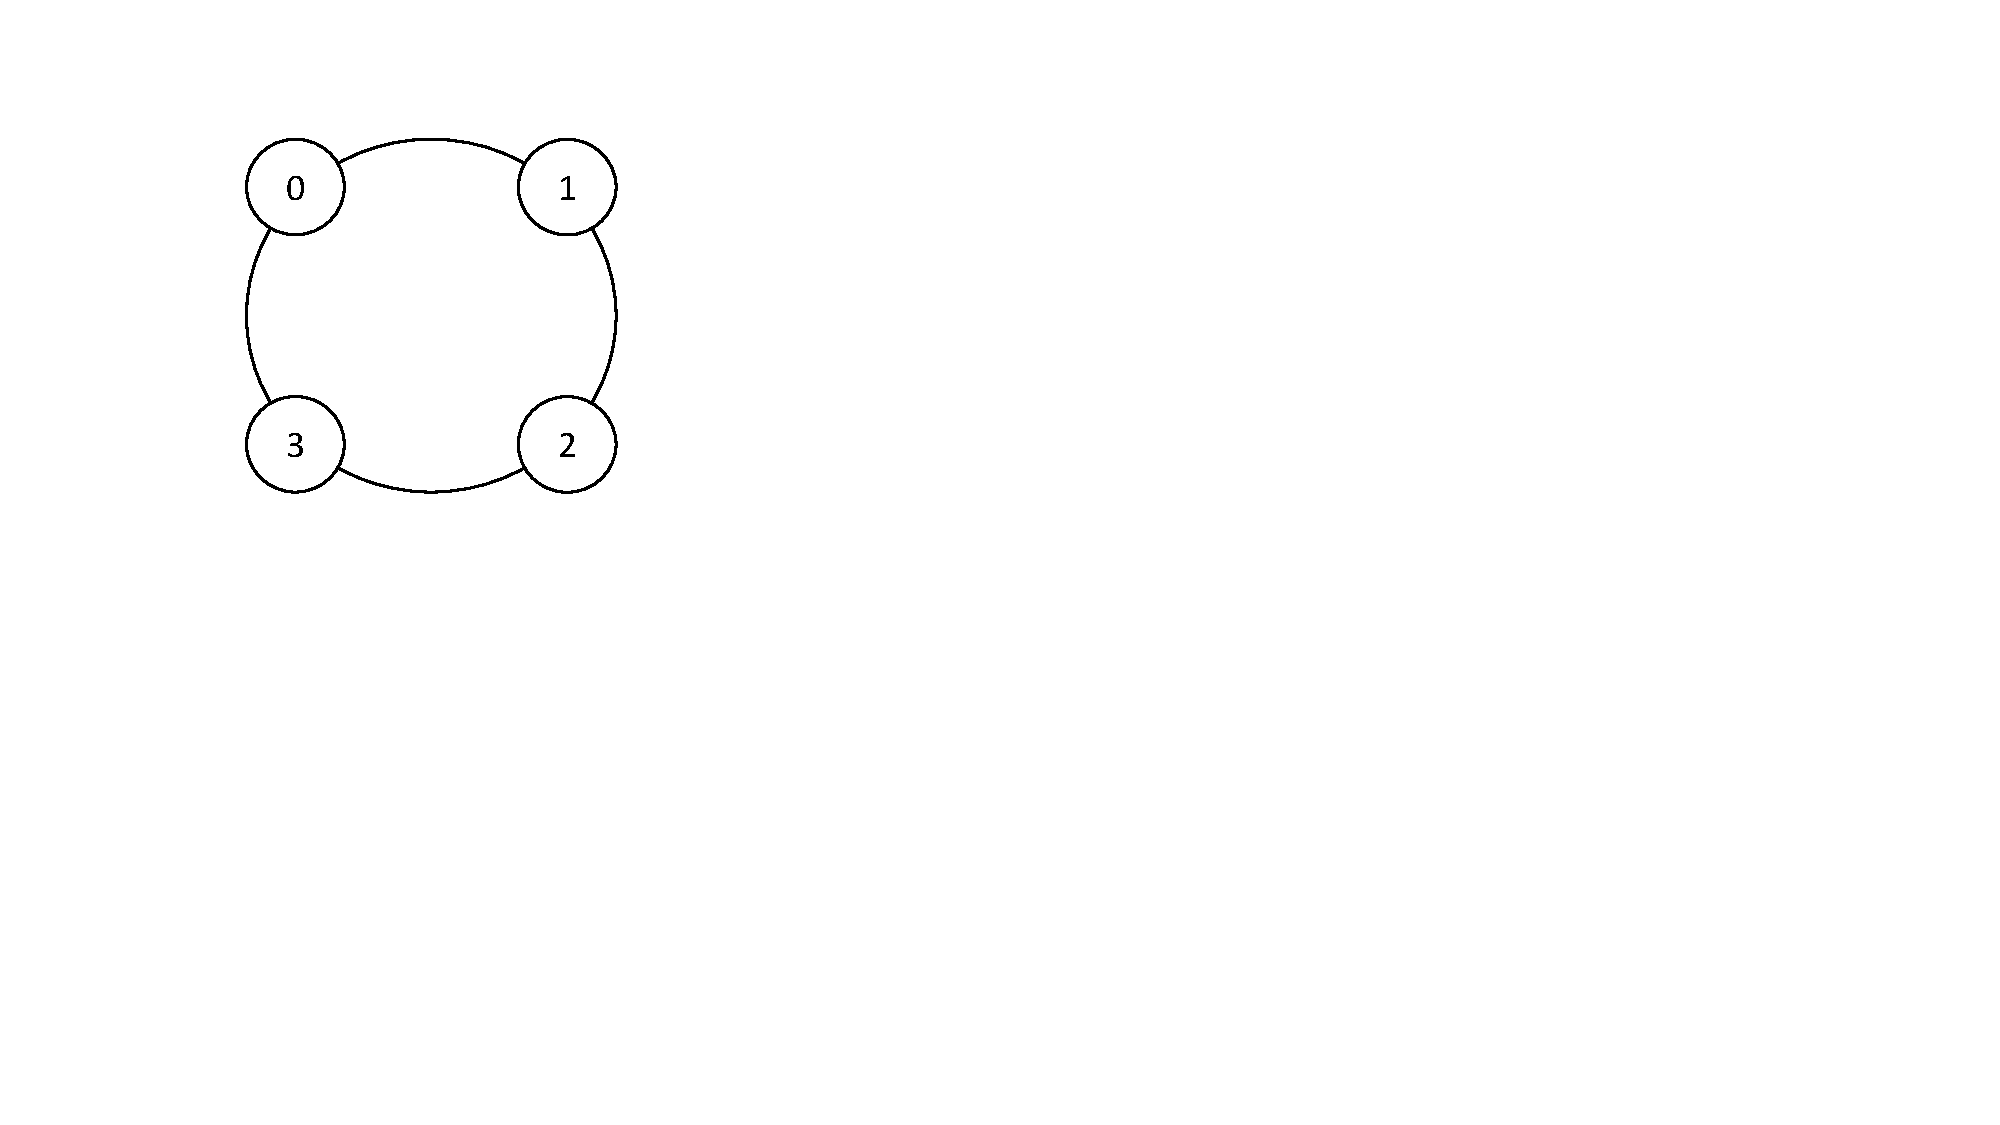
\includegraphics[width=.4\linewidth]{Example-Bubbles.pdf}
\captionof{figure}{Illustrative Example}
\label{fig:illustrative_example}
\end{center}

\noindent \textbf{An Illustrative Example} We illustrate our model with a simple example. Suppose that there are four products: 0, 1, 2, 3. The products are in different places of the product space, where 1 is close to 0 and 2 but more distant from 3, as shown in Figure \ref{fig:illustrative_example}.
Suppose that the user actually believes that they all have expected value of 0 and consumes product 1. The underlying correlation structure implies that upon observing that $x_1=y$ the user will update beliefs about $\mathbb E x_0$, $\mathbb E x_2$ and $\mathbb E x_3$ to $\rho y$, $\rho y$ and $\rho^2 y$ respectively. This is because learning about product 1's value is more informative about similar products' value, 0 and 2, than products further away in the product space, 3. Therefore, the user will adjust her beliefs about their mean -- zero in the example -- more strongly for products which are similar. Moreover, now uncertainty about the value of products 0, 2 and 3 is also decreased but differentially so: learning product 1's value has contributed to a stronger reduction of uncertainty for nearby products that for product 3. If the actual value was positive, this induces the user to perform some local exploration, as 0 and 2 have higher mean and lower variance. If instead it was negative, then user's posterior beliefs penalize more strongly products 0 and 2 than 3, so if she is not too risk averse, she would go across the product space in search of some better element. However, if risk aversion is high enough, the user might be willing to trade-off ex-ante expected lower values for lower risk and stick to local exploration of products that have just because the user has less uncertainty about their values. As the saying goes, if you are risk-averse, better the devil you know.
\par

\noindent \textbf{Recommendation}
Our model of recommendation is stylized in order to provide qualitative insights into how recommendation shapes behavior, instead of focusing on the details of how recommender systems are implemented in practice. We model recommendation as giving users information about the valuation of the products.
\par

We will consider three cases. The case of primary interest is \textit{recommendation} where the recommender observes values accrued and knows $V$ but does not know neither $V_i$.\footnote{We do not consider the acquisition of information for the recommender to know $V$ and suppose that she has sufficient data to learn $V$ with arbitrary precision.} However, the recommender does know the users' beliefs $\bar V_i$. Thus, at any given period, the recommender provides a personalized recommendation that combines the knowledge of the common value component $V$ with the user beliefs $\bar V_i$. Knowing the user's beliefs about her valuation of each item become crucial in this case: just providing the user with information about $V$ may change the user's original ranking, but, without considering the user's beliefs, she will not necessarily follow the recommendation.
\par

The notion of recommendation that we consider is idealized where the recommendation does the Bayesian updating for users. As users face a very difficult and costly Bayesian updating instance, a useful recommendation system provides recommendations taking into account this aspect and combines the history of past consumption and value realizations with the user's beliefs. 
An alternative that is equivalent would be the recommender simply providing $V$ without knowing $V_i$. In this case, the recommendation will be that the user $i$ chooses $r_{i,t} \in \arg \max_{n\in \mathcal J\backslash C^T_i} \mathbb E[u(x_n) \mid C_i^T]$
but we assume the recommender provides full information about $V$. \footnote{For instance, the recommender could display the whole distribution of utilities reported by other users or even its average, which is a good proxy for the common value component. It is possible for the recommender to only recommend the best item given such information, that is, the item with highest common value component. However, in that case, recommending only a single item generates costly Bayesian updating to the user and provides little guidance as to what she should indeed pick as the common value might be of little importance when compared to the idiosyncratic component. Therefore, we assume that the recommender reports the whole $V$, which results in higher expected welfare in choices and is not costly to implement.}
The results would be equivalent, but this would shift the burden of Bayesian updating to users.
\par

We further consider two cases that serve primarily as benchmarks. The first is \textit{no recommendation}, where users get no additional information about utilities and make consumption choices based on their beliefs and consumption history. This gives us a benchmark as to how users in our model would behave \textit{without} recommendation so that we can analyze what changes with the introduction of recommendation. The second is the \textit{oracle recommendation} where the recommender knows the true realized utility of each good for each user and can therefore recommend the best remaining good in every period. This gives us a full information benchmark, which is the optimal consumption path for a user if all uncertainty about their preferences was resolved.
\par

\noindent \textbf{Simulation Details}. 
We analyze our model using numerical simulation since the sequential decision-making component of our model paired with the rich covariance structure between the items make it difficult to characterize optimal user behavior analytically. The Gaussian assumption allows for closed form Bayesian-updating which enables us to simulate our model but does not provide much help in analytical characterizations. 
\par

We explore how consumption patterns differ as we consider different recommendation regimes and report representative results from our simulations. We simulate our model over 100 populations of users with 100 users per population. For every population and every statistic we calculate, we average over the users in the population to get a representative statistic for this population. A given set of parameters and a population are a single data point in our dataset.
\par

We simulate over risk-aversion parameters $\gamma \in \{ 0, 0.3, 0.6, 1, 5 \}$, standard-deviation $\sigma \in \{ 0.25, 0.5, 1.0, 2.0, 4.0 \}$, correlation parameters $\rho\in \{ 0, 0.1, 0.3, 0.5, 0.7, 0.9 \} $ and degree of idiosyncrasy of individual valuations $\beta \in \{ 0, 0.4, 0.8, 1, 2, 5\}$. When we consider results varying a single parameter, we group the results over the other parameters and provide reports varying only the parameter of interest. We report results for a relatively small consumption history $T=20$ with a produce space size $N=200$. Unless otherwise reported, our results are robust to varying $N$.

\subsection{Discussion of the Assumptions}
In this section we provide further discussion of several assumptions of our model.
\par

\noindent \textbf{Uncertainty}: We assume that users have underlying uncertainty about the realized value of the items in their choice sets and as a result face a decision problem under uncertainty. The first justification for this is that environments where recommender systems are commonly deployed, such as on media streaming and e-commerce platforms, are mostly dedicated to experience goods, where users only learn their value after consumption. Standard decision theory axiomatized the conditions under which behavior is described by (subjective) expected utility maximizers \cite{savage1954} who update beliefs according to Bayesian inference \cite{ghirardato2002revisiting}, to which we add the assumption that their prior is correct. The second justification is that, even if users are in an environment where they could observe utilities based on product reviews or introspection, it is prohibitively costly for them to do so in large choice sets.\footnote{Recent empirical work \cite{bronnenberg2014zooming,hodgson2019horse} has shown that, for product search, users engage in a ``zooming in'' search strategy in terms of the information they acquire about products before purchasing and only end up acquiring information about a small set of products in a large product space}  Even if they acquired all the information from product reviews, this would not fully resolve uncertainty as to the extent that individuals have idiosyncratic tastes. Giving that users are facing choices problems uncertainty, this motivates modeling recommendation as providing users \textit{information} in order to reduce their uncertainty.
\par

\noindent \textbf{Large Choice Sets}: We are interested in environments where the number of items in the choice set is large and users only consume a small number of these items. This is realistic for platforms such as Netflix, Spotify, Amazon and YouTube where there are sometimes billions of items and users can realistically only consume a handful of these items in their lifetime.\par

\noindent \textbf{Learning Spillovers}: Users in our environment face a sequential decision-making problem. However, we suppose that individuals are myopic, i.e. they consume the item with the highest expected utility given their beliefs at each period. This is assumed in order to preserve tractability. The predominant difficulty in the learning problem they face is not that they need to repeatedly sample a single item in order to learn its value as in the standard multi-armed bandit formulations, but rather that they need to be able to generalize from their experience from consuming one item to other items. After consuming a single item, they learn the realized value of the good, but have no desire to consume it again, i.e. we assume that there is no value to consuming the item again.
\par

\cite{schulz2019structured} studies how individuals solve sequential decision-making problems under uncertainty in large choice sets in the context of mobile food delivery orders. They find that individuals engage in similarity-based generalizations where learning about the realized value of a particular good provides them with information about similar goods. Content-based recommender systems exploit a similar idea where, if a user liked a given item, then she is also likely to like a similar but different item as well.
\par

Our model incorporates this observation in a stylized fashion, where the degree of information spillovers is controlled via parameter $\rho$ and we study how the strength of the spillovers impacts behavior and the effect of recommendation.
\par

\section{Results}
\subsection{Local Consumption}
\begin{figure}
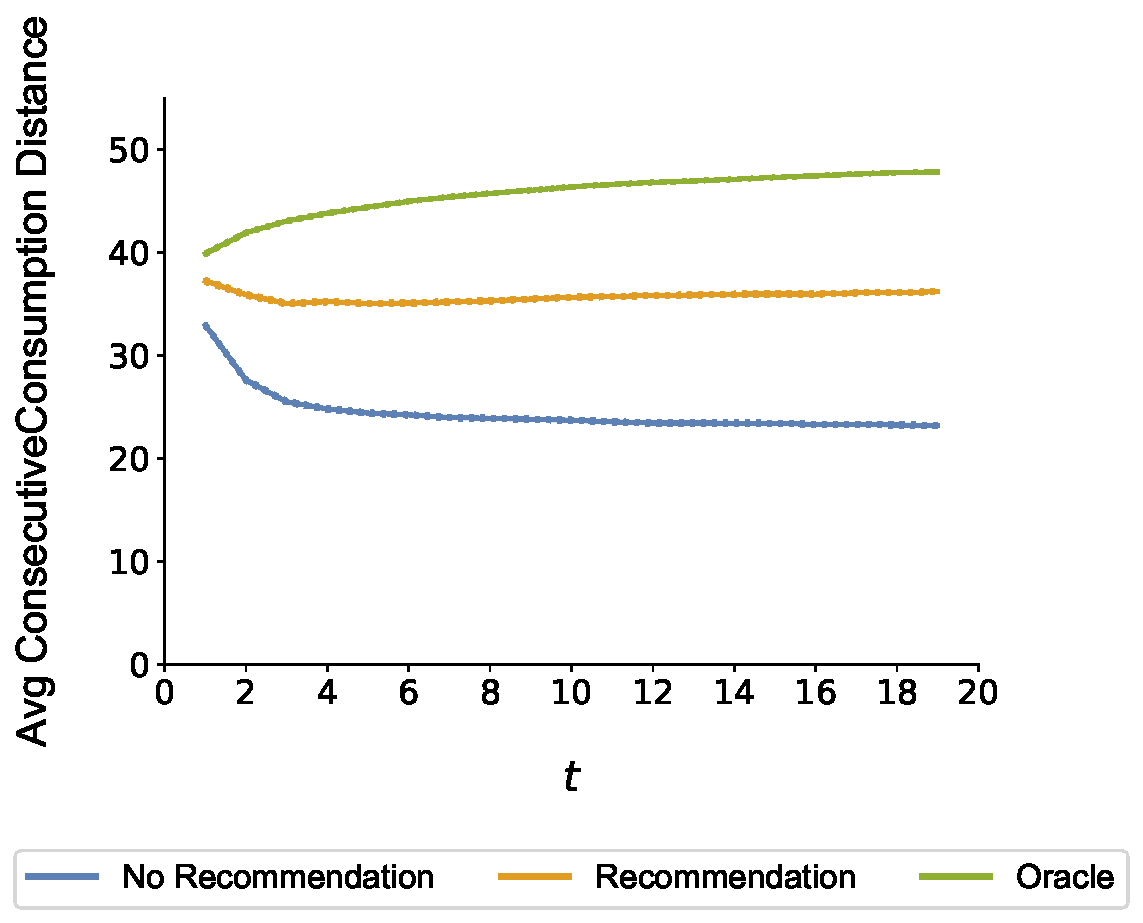
\includegraphics[width=.9\linewidth]{figures/rho_pos_consumption_dist_N_200T_20_overall.pdf}\\
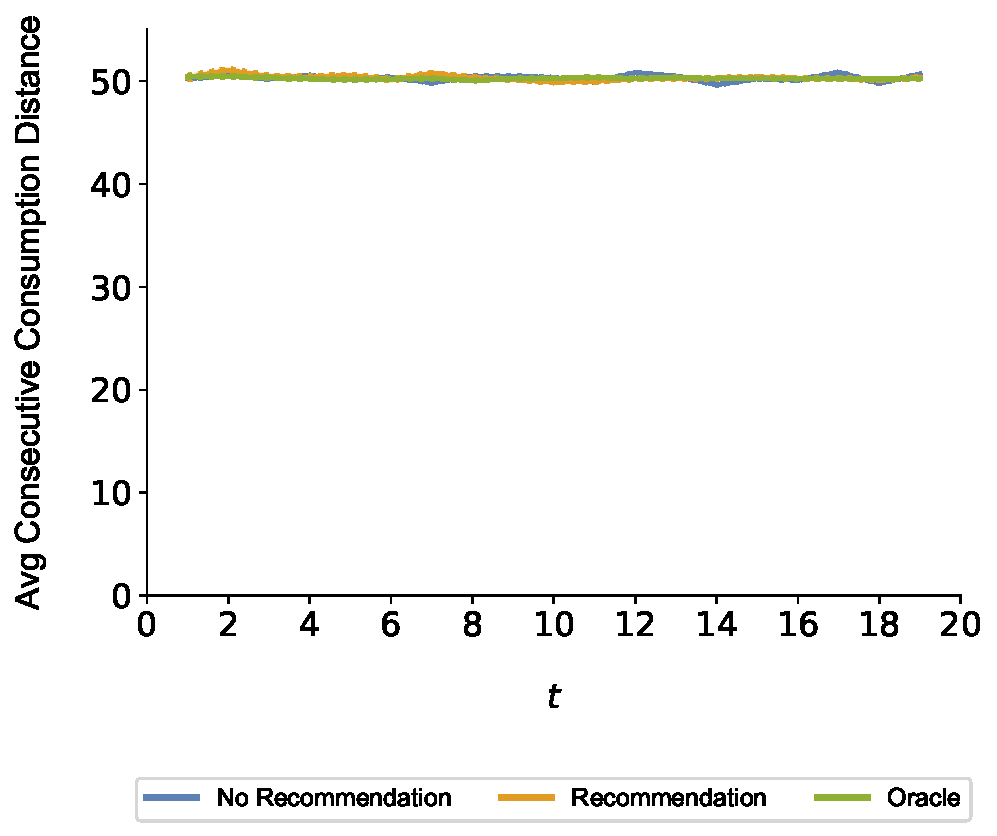
\includegraphics[width=.9\linewidth]{figures/rho_zero_consumption_dist_N_200T_20_overall.pdf}\\
\caption{Consumption path with (Top) and without (Bottom) correlation between values}
\label{fig:correlation_consumption_path}
\end{figure}

We characterize ``filter bubble'' effects in our model as the degree to which users engage in \textit{local consumption}. We define local consumption in terms of the average consumption distance between the items consumed by the users at time $t-1$ and $t$. We compare the average movement within the product space across different recommendation regimes and associate lower average distance with more local consumption.

\begin{finding}\label{finding_local_consumption}
The impact of recommendation on local consumption:
\begin{enumerate}
\item When $\rho = 0$, there is no difference in consumption distance between the three recommendation regimes.
\item When $\rho > 0$, no recommendation induces more local consumption than both recommendation and oracle regimes. This effect is amplified as $\rho$ increases as well as when users are more risk averse ($\gamma$ increases)
\end{enumerate}
\end{finding}

First, the bottom panel of Figure \ref{fig:correlation_consumption_path} shows that, when $\rho = 0$, there is no difference in consumption distance between the three regimes. This is due to the fact that when $\rho = 0$, there is no reason that items that are close in the product space should have similar utilities and so the optimal consumption path does not depend on the similarity of the items. However this also means that users do not learn anything about neighboring products and so there is limited path-dependence in consumption.
\par

The top panel of Figure \ref{fig:correlation_consumption_path} shows that, when $\rho > 0$, both recommendation and no recommendation lead to increasingly local consumption compared to the oracle benchmark case. Further, the average consumption path between periods is \textit{decreasing} for the no recommendation case whereas it is \textit{increasing} for the oracle case. The recommendation regime decreases the degree of local consumption but not as much as the oracle benchmark. Due to the correlation of values, the oracle consumption path exploits this and leads to the consumption of more similar products than in the case when $\rho = 0$. However, since these spillovers also impact user learning in the no recommendation case, users \textit{over-exploit} this and increasingly consume products similar to good products that they have consumed before. This is further illustrated by Figure \ref{fig:local_consumption_across_rho} which shows how the consumption paths in the oracle and no recommendation regimes vary as $\rho$ increases.
\par

Finally, this effect is further amplified as the level of risk aversion, $\gamma$, increases. Figure \ref{fig:no_rec_risk_aversion} shows how drastically the degree of local consumption increases as $\gamma$ increases. This is due to the fact that the spillovers not only affect the mean expected belief about quality but also the degree of uncertainty. Local consumption therefore leads to users having less uncertainty about certain areas of the product space and risk aversion may lead them to increasingly consume nearby products.

\begin{figure}[t]
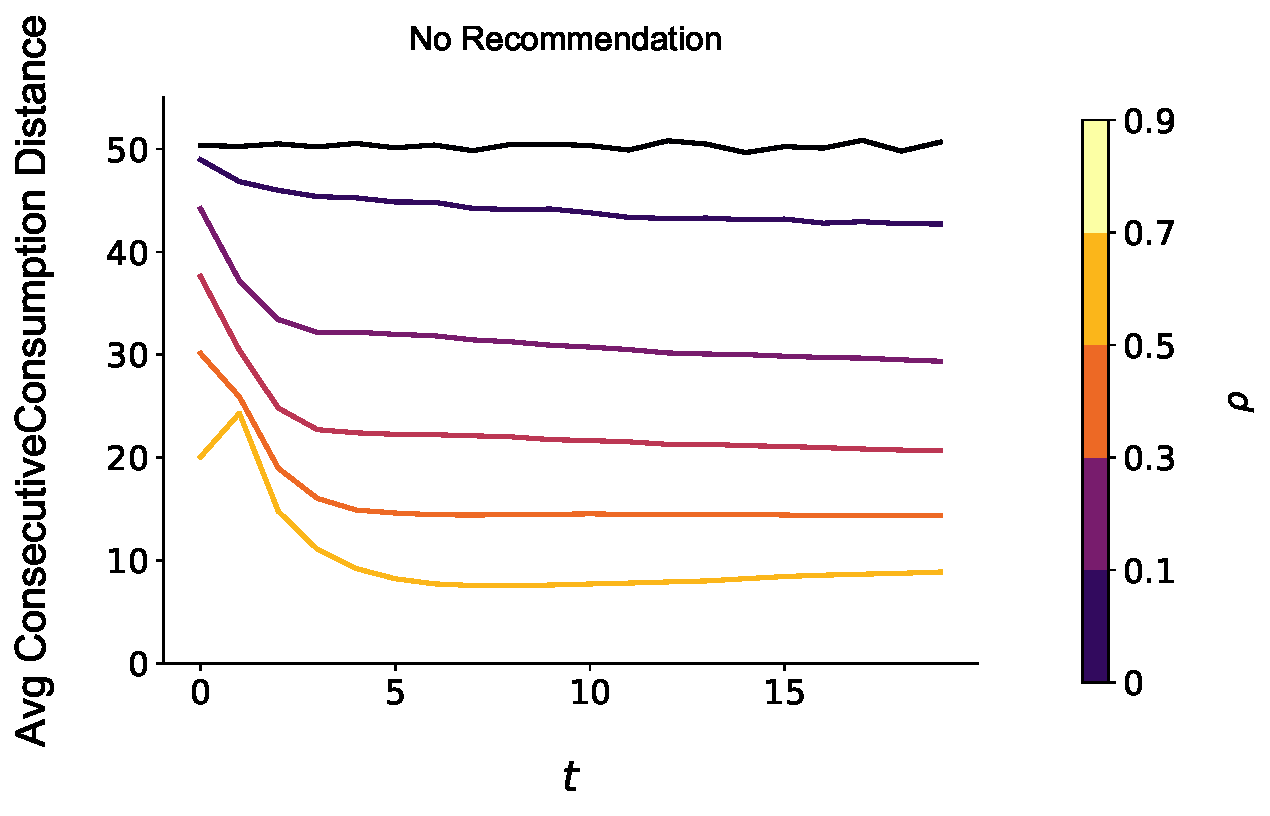
\includegraphics[width=\linewidth]{figures/rho_consumption_dist_N_200T_20.pdf}\\
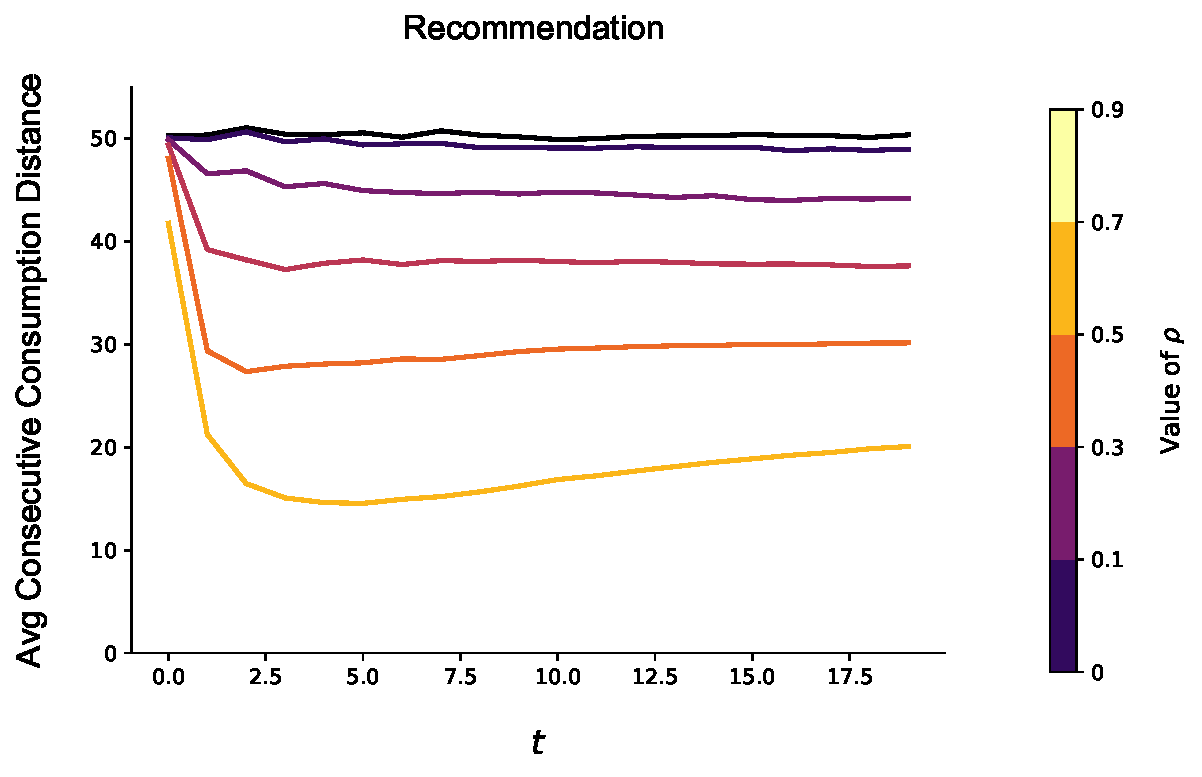
\includegraphics[width=\linewidth]{figures/rho_consumption_dist_N_200T_20_partial.pdf}\\
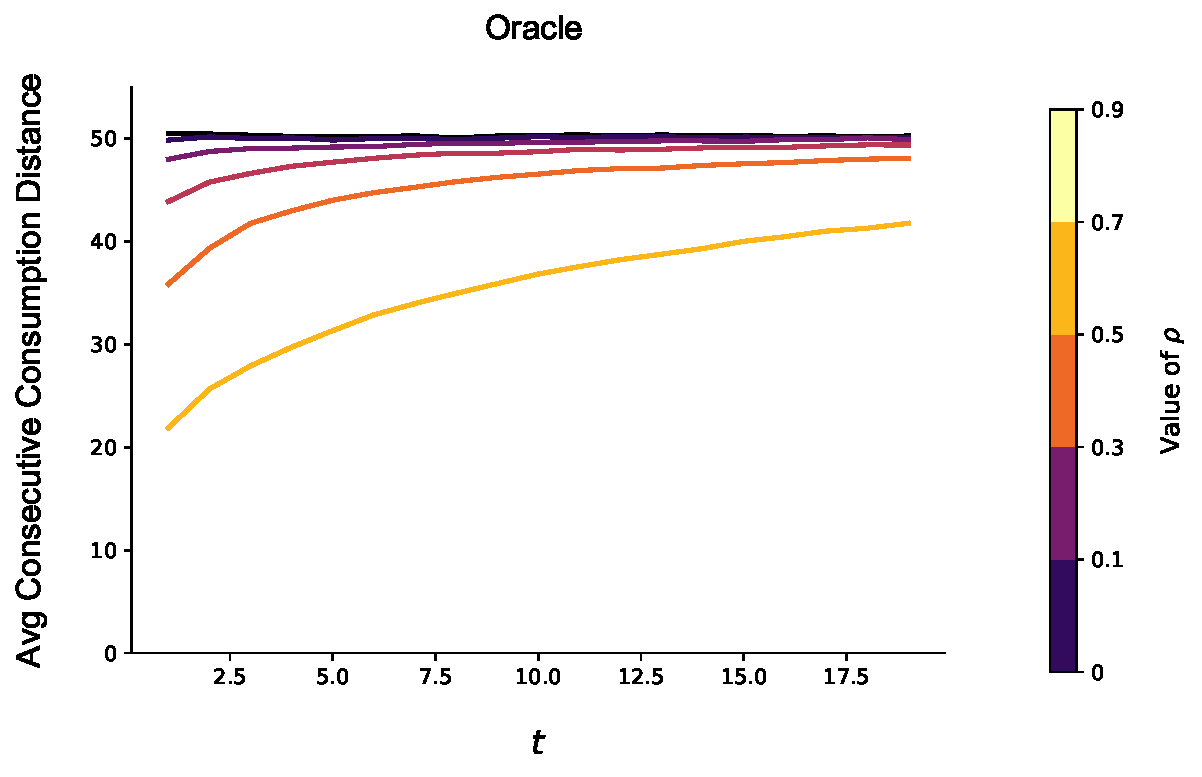
\includegraphics[width=\linewidth]{figures/rho_consumption_dist_N_200T_20_omni.pdf}\\
\caption{Extent of Local Consumption for No Recommendation (Top), Recommendation (Middle) and Oracle (Bottom) for different Correlation values}
\label{fig:local_consumption_across_rho}
\end{figure}

\begin{figure}[t]
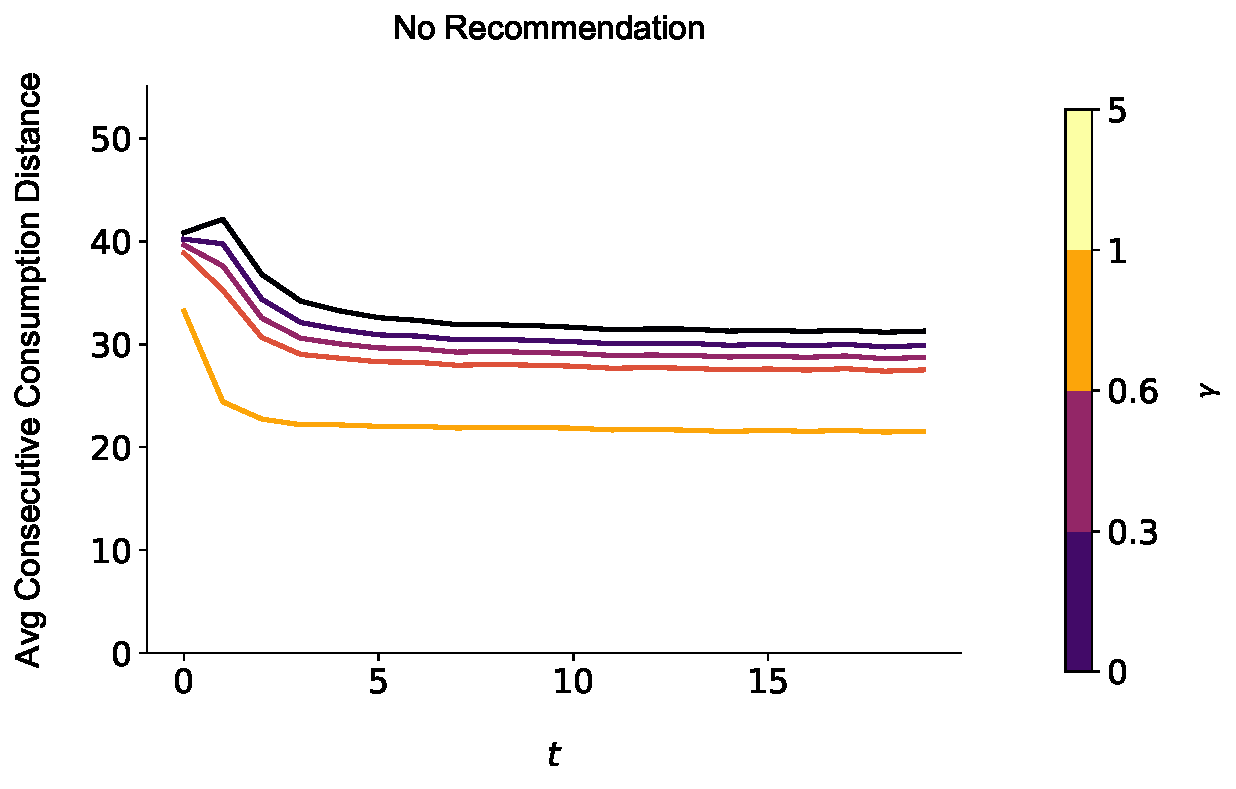
\includegraphics[width=\linewidth]{figures/gamma_consumption_dist_N_200T_20.pdf}\\
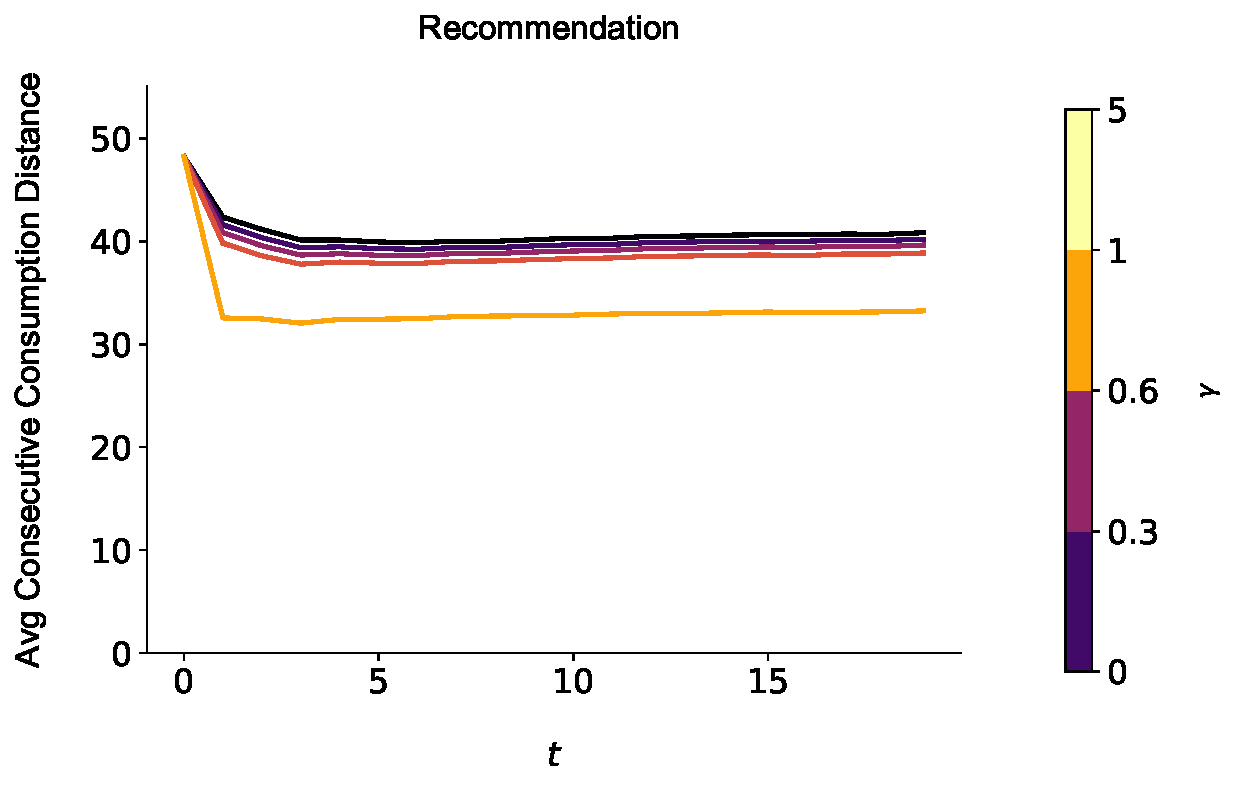
\includegraphics[width=\linewidth]{figures/gamma_consumption_dist_N_200T_20_partial.pdf}\\
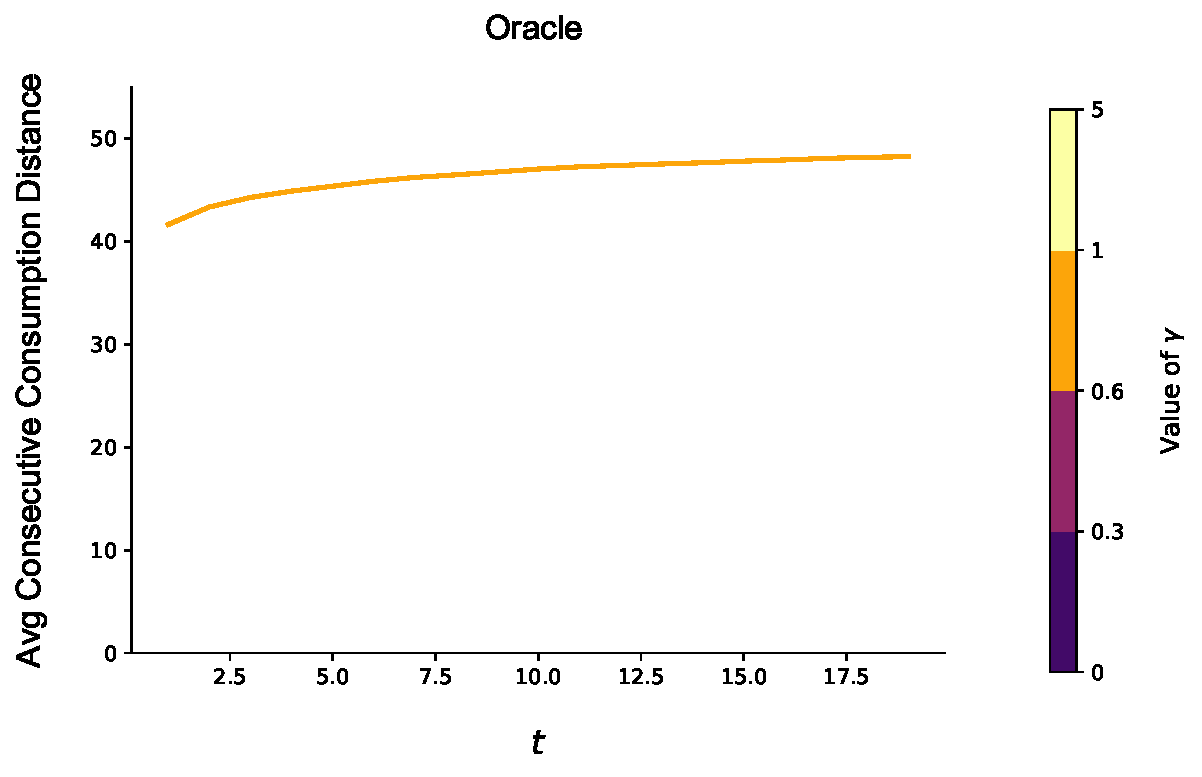
\includegraphics[width=\linewidth]{figures/gamma_consumption_dist_N_200T_20_omni.pdf}\\
\caption{Effect of Risk Aversion on Local Consumption for No Recommendation (Top), Recommendation (Middle) and Oracle (Bottom)}
\label{fig:no_rec_risk_aversion}
\end{figure}

In sum, in our model filter bubbles are driven by learning-spillovers and risk aversion. It is the belief that there is an underlying correlation across different products' values, stronger for similar products, closer in the product space, that leads users to focus on local consumption upon consuming high valued items. For instance, upon discovering that the user likes movies by a given director, she will be more likely to explore other movies by the same director. Risk aversion may lead users into performing local consumption even when they have a low valuation of nearby products just because they know what to expect from the product.
\par

\subsection{User Welfare and Product Diversity}
In this section we primarily focus on the impact of recommendation on the welfare on users as well as the overall diversity of the items that they consume. We define user's \textit{ex-post} welfare as the average of the realized values, controlling for the effect of $T$
$$W_i:= \frac{1}{T}\sum_{n \in C_i^T} x_{i,n}$$

While in the previous section we looked at the distance between consecutive goods, we also define a diversity measure that is defined over the entire consumed set. We utilize a diversity metric common in the literature (e.g. \cite{ziegler2005improving}) which is the average normalized pairwise distance between the consumed products:
$$D_i:=\frac{1}{N}\frac{1}{T(T-1)}\sum_{n,m \in C_i^T: n \ne m} d(n,m)$$

\begin{finding}\label{finding_diversity}
The impact of recommendation on product diversity:
\begin{enumerate}
\item When $\rho = 0$, product diversity is the same across all three recommendation regimes;
\item When $\rho > 0$, product diversity decreases across all recommendation regimes but decreases the most in the no recommendation regime. This effect is amplified as $\rho$ increases as well as when users become more risk-averse.
\end{enumerate}
\end{finding}

As before, when there is no correlation between utilities product diversity is the same across different recommendation regimes. The over-exploitation of the learning spillovers when $\rho > 0$ leads to product diversity being lowest in the no recommendation regime.  Figure \ref{fig:risk_aversion_diversity} shows how diversity varies as risk aversion levels change and Figure \ref{fig:diversity_correlation} shows how diversity varies across recommendation regimes and the level of $\rho$.

\begin{figure}[ht]
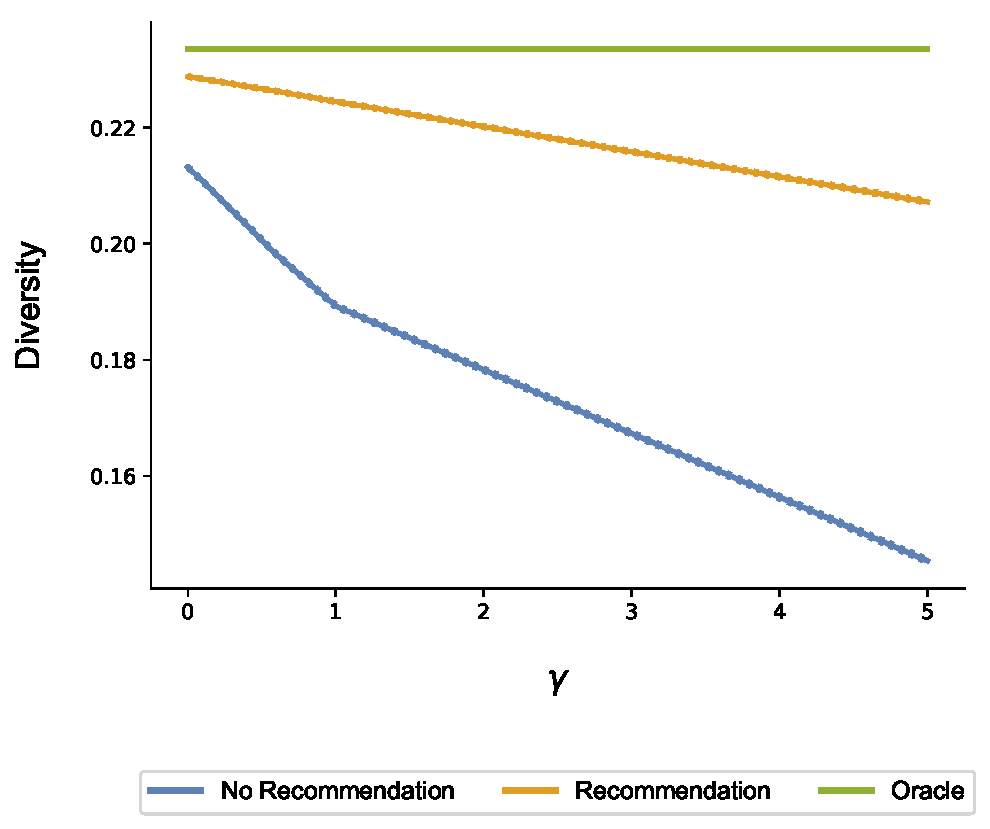
\includegraphics[width=.9\linewidth]{figures/gamma_diversity_N_200_T_20}
\captionof{figure}{Risk Aversion and Diversity}\label{fig:risk_aversion_diversity}
\end{figure}

\begin{finding}\label{finding_welfare_gap}
The welfare gap between the no recommendation and the recommendation regimes and that between the no recommendation and the oracle regimes are decreasing in $\rho$.
\end{finding}
However, interestingly, the decrease in diversity is \textit{not} associated with a decline in welfare. In fact, welfare stays roughly the same in the oracle and recommendation cases. The welfare gap between the no recommendation case and the other two cases \textit{decreases} as the diversity gap increases.
\par
\begin{figure}[t]
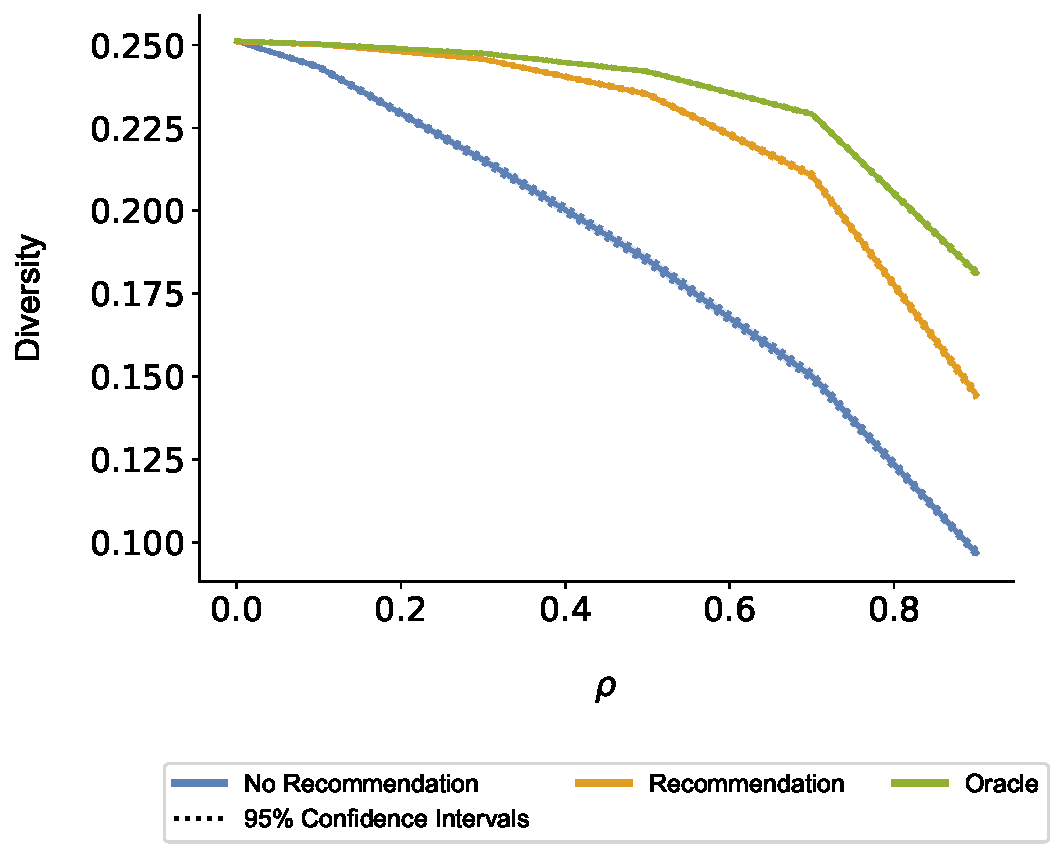
\includegraphics[width=.9\linewidth]{figures/rho_diversity_N_200_T_20.pdf}\\
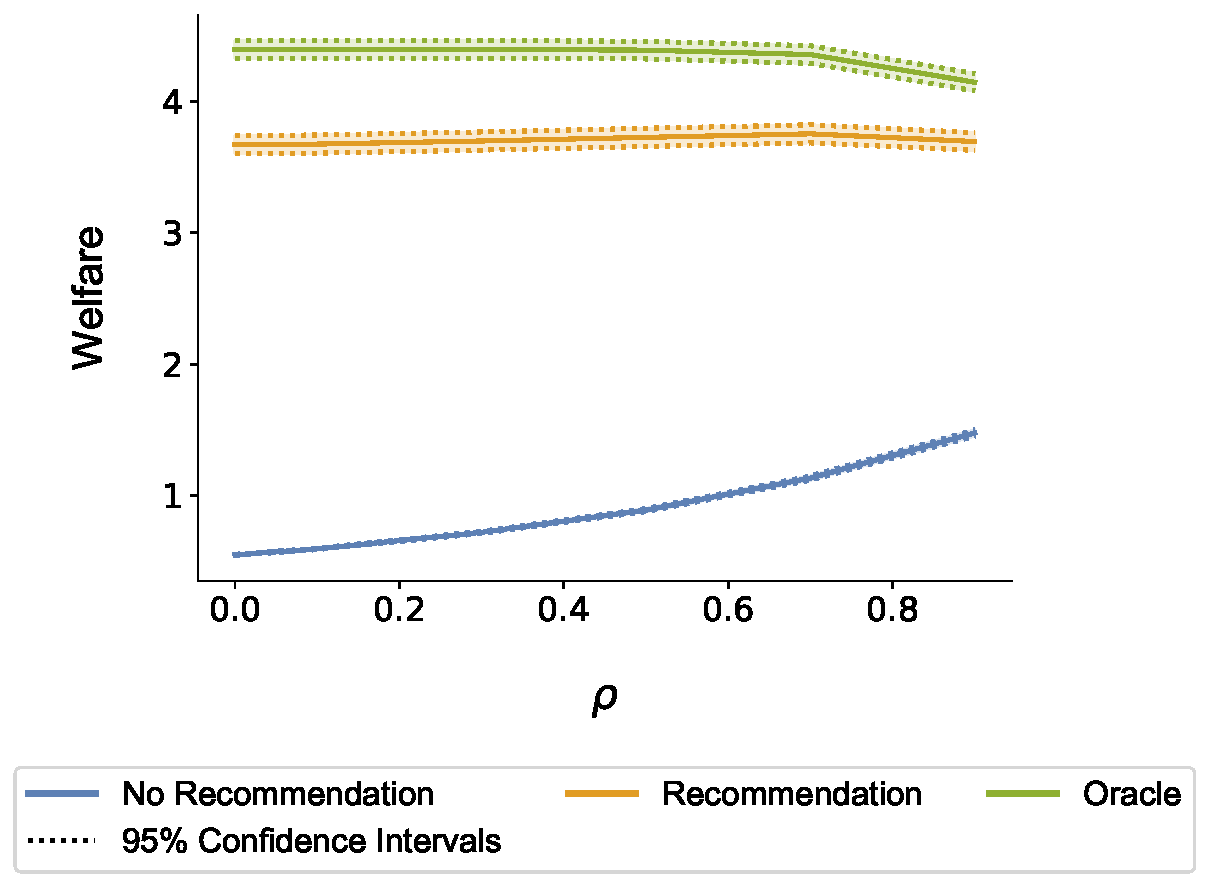
\includegraphics[width=.9\linewidth]{figures/rho_welfare_N_200_T_20.pdf}\\
\captionof{figure}{Welfare, Diversity, and Correlation}\label{fig:diversity_correlation}
\end{figure}

\begin{finding}\label{finding_diversity_welfare_corr}
In the no recommendation regime, diversity and welfare are:
\begin{enumerate}
\item Negatively correlated when users have no risk-aversion;
\item Uncorrelated when users have high levels of risk-aversion.
\end{enumerate}
In the recommendation regime, diversity and welfare are:
\begin{enumerate}
\item Uncorrelated when users have no risk-aversion;
\item Positively correlated when users have high levels of risk-aversion.
\end{enumerate}
In the oracle regime, diversity and welfare are always uncorrelated.
\end{finding}

Figure \ref{fig:diversity_welfare_ra} shows how diversity and welfare correlate for the no recommendation case. When there is no risk-aversion then there is a negative correlation between welfare and diversity. This is since, with no risk-aversion, in a given period a user will select the good that she currently believe has the highest expected value. High product diversity in this case can arise from a user who consumes an item she disliked and updates her beliefs about nearby items negatively. As a result, in the following period she will pick an item far away in the product space from the item that was previously consumed. If instead the user valued highly the item that she had consumed, then she is more likely to pick a nearby item. The learning spillovers therefore lead to high product diversity being negatively correlated with welfare.
\par



%\begin{figure}

%\end{figure}

This only happens since $\gamma = 0$ leads to users only caring about the expected value of the product. However, as we saw in Findings \ref{finding_local_consumption} and \ref{finding_diversity}, increasing $\gamma$ can lead to lower diversity and increasingly local consumption due to the fact that the degree of uncertainty now impacts users' choices. This weakens the negative relationship between diversity and welfare since both negative and positive experiences with a good reduce uncertainty about surrounding goods. This leads to the inverted-U shape found in Figure \ref{fig:diversity_welfare_ra} when $\gamma$ is relatively large (e.g $\gamma = 5$) though diversity and welfare are virtually uncorrelated in the data. In the recommendation and oracle regimes, under risk neutrality ($\gamma=0$), welfare and diversity and uncorrelated, while under risk aversion ($\gamma=5$), it is possible to observe in Figure \ref{fig:diversity_welfare_ra_partial} an actual positive relation between diversity and welfare as recommendations are able to reduce uncertainty and facilitate exploration of the product space.
\par
\begin{figure}[t]
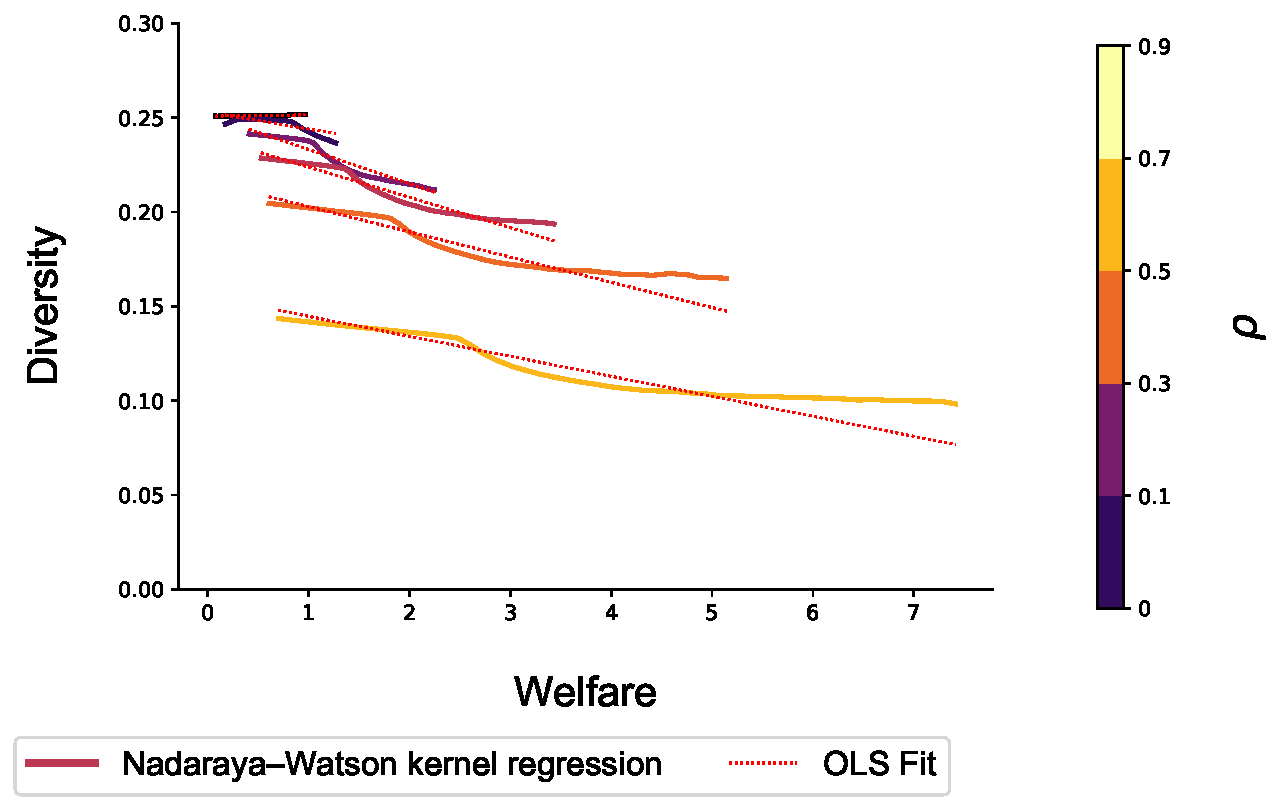
\includegraphics[width=1.05\linewidth]{figures/diversity_welfare_rn.pdf}\\
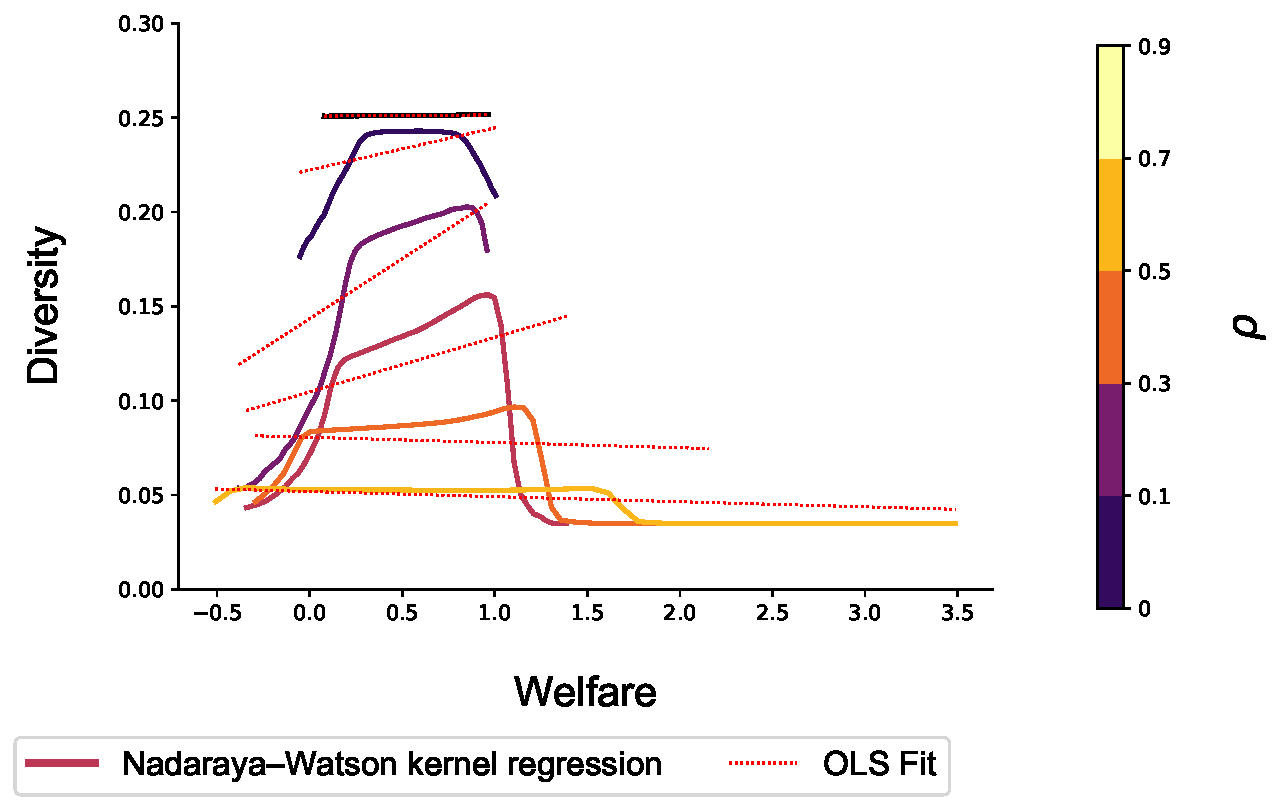
\includegraphics[width=1.05\linewidth]{figures/diversity_welfare_ra.pdf}\\
\captionof{figure}{Diversity vs. Welfare, No-Recommendation, $\gamma = 0$ (Top), Diversity vs. Welfare, $\gamma = 5$ (Bottom)}\label{fig:diversity_welfare_ra}
\end{figure}
\begin{figure}[t]
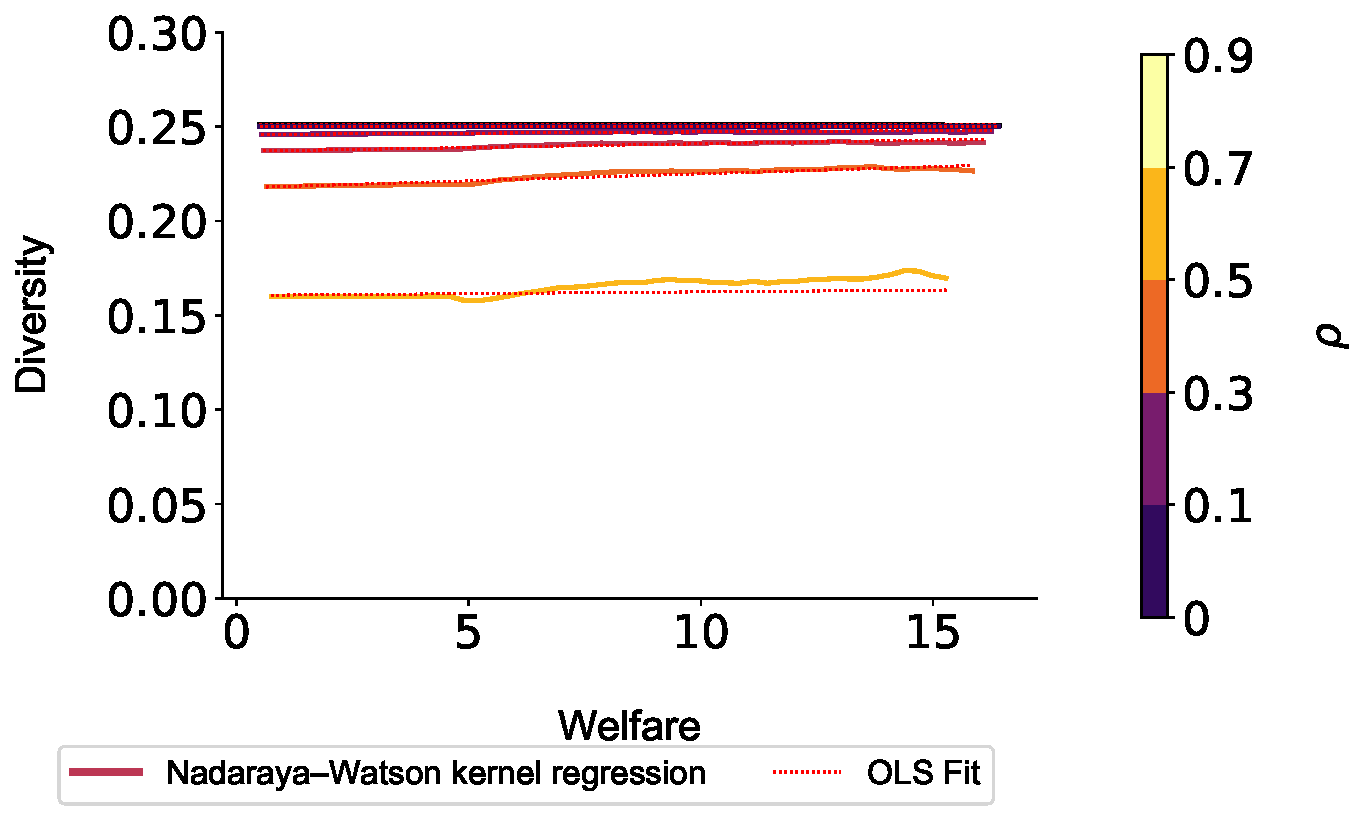
\includegraphics[width=1.05\linewidth]{figures/diversity_welfare_rn_partial.pdf}\\
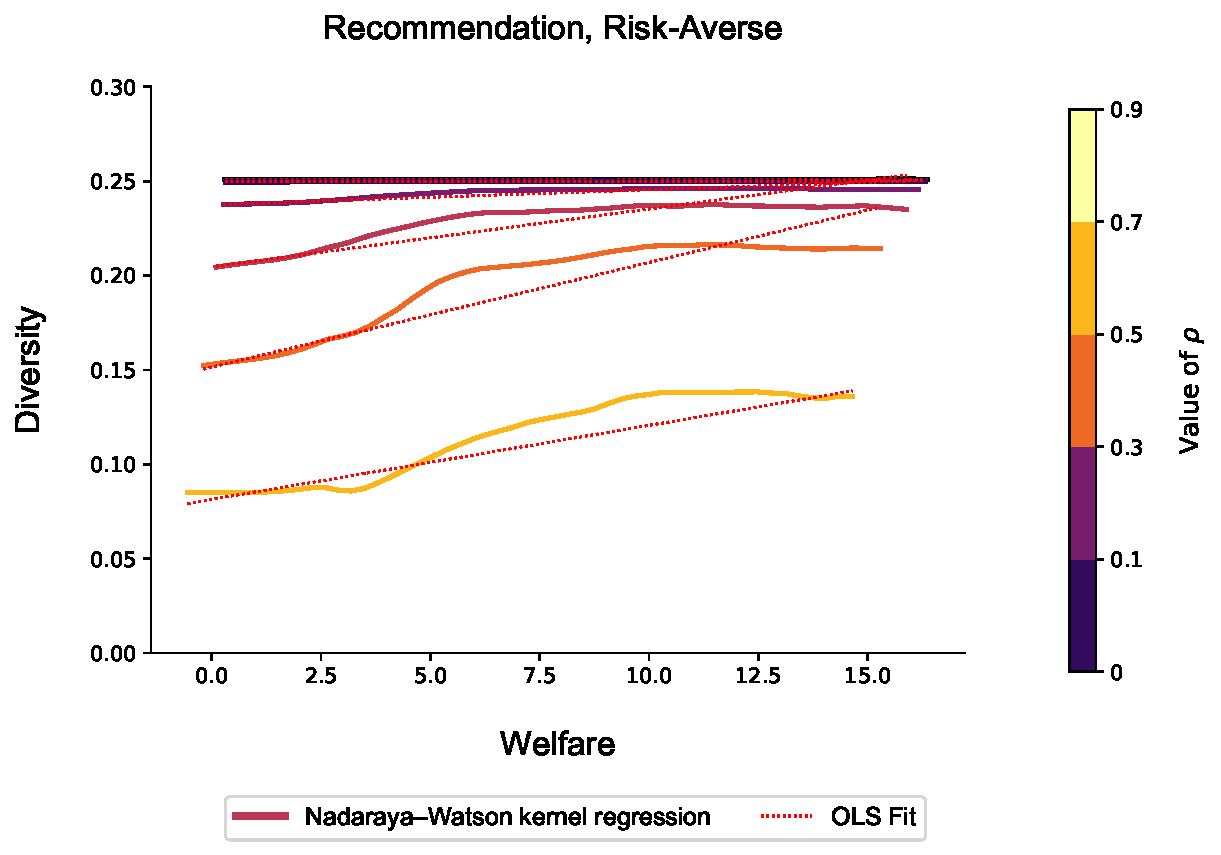
\includegraphics[width=1.05\linewidth]{figures/diversity_welfare_ra_partial.pdf}\\
\captionof{figure}{Diversity vs. Welfare, Recommendation, $\gamma = 0$ (Top), Diversity vs. Welfare, $\gamma = 5$ (Bottom)}\label{fig:diversity_welfare_ra_partial}
\end{figure}

\subsection{User Homogenization}
In this section we focus on across user comparisons and investigate how the consumed set of items across users varies across different recommendation regimes and parameter values. In particular we look at the degree of \textit{homogenization} between users. Similar to \cite{chaney2018algorithmic} we use the Jaccard index between the consumption sets of users to measure homogeneity:
\begin{align*}
H:=\frac{1}{|I|(|I|-1)}\sum_{i,j \in I: i \ne j}d_J(C_i^T,C_j^T)
\end{align*}
where $d_J$ denotes the Jaccard index and $H \in [0,1]$.
\begin{finding}\label{finding_homogeneity}
Homogeneity is:
\begin{enumerate}
\item Highest under recommendation and lowest under no recommendation;
\item Increasing in $\beta$, or the weight of the common-value component;
\item Decreasing in $\rho$ for partial recommendation, but weakly increasing in $\rho$ for no recommendation.
\end{enumerate}
\end{finding}
Figure \ref{fig:beta_homo} shows that as the weight of the common-value component, $\beta$, increases users consume increasingly similar sets of items. The homogenization effect is strongest under the recommendation regime since the revelation of the common-value component induces users to consume products in similar areas of the product space. However, as $\beta$ increases, some amount of homogenization is optimal as can be seen from the oracle case. In the no recommendation regime since users do not know the common-value component they engage in local consumption in different areas of the product space which leads to less than optimal homogeneity.
\par

Figure \ref{fig:cor_homo} shows that the degree of homogeneity in the recommendation case however is \textit{decreasing} as $\rho$ increases. As was highlighted in Findings \ref{finding_local_consumption} and \ref{finding_diversity}, the degree of local consumption increases with $\rho$. Even though the revelation of the common-value component induces them to search in similar parts of the product space, their idiosyncratic components induce them to consume products in a more localized area of the product space as $\rho$ increases which leads to a decline in homogeneity.

\begin{figure}[t]
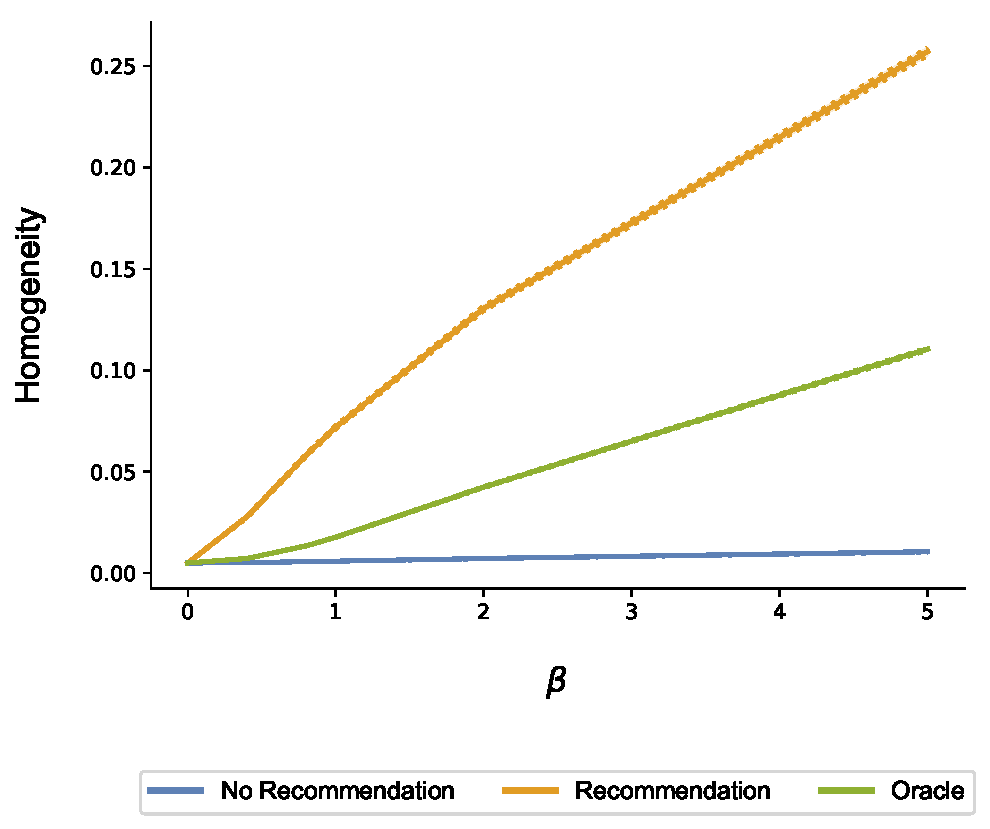
\includegraphics[width=.8\linewidth]{figures/beta_homogeneity_N_200_T_20}
\captionof{figure}{Strength of Recommendation and Homogeneity}\label{fig:beta_homo}
\end{figure}
~

\begin{figure}[t]
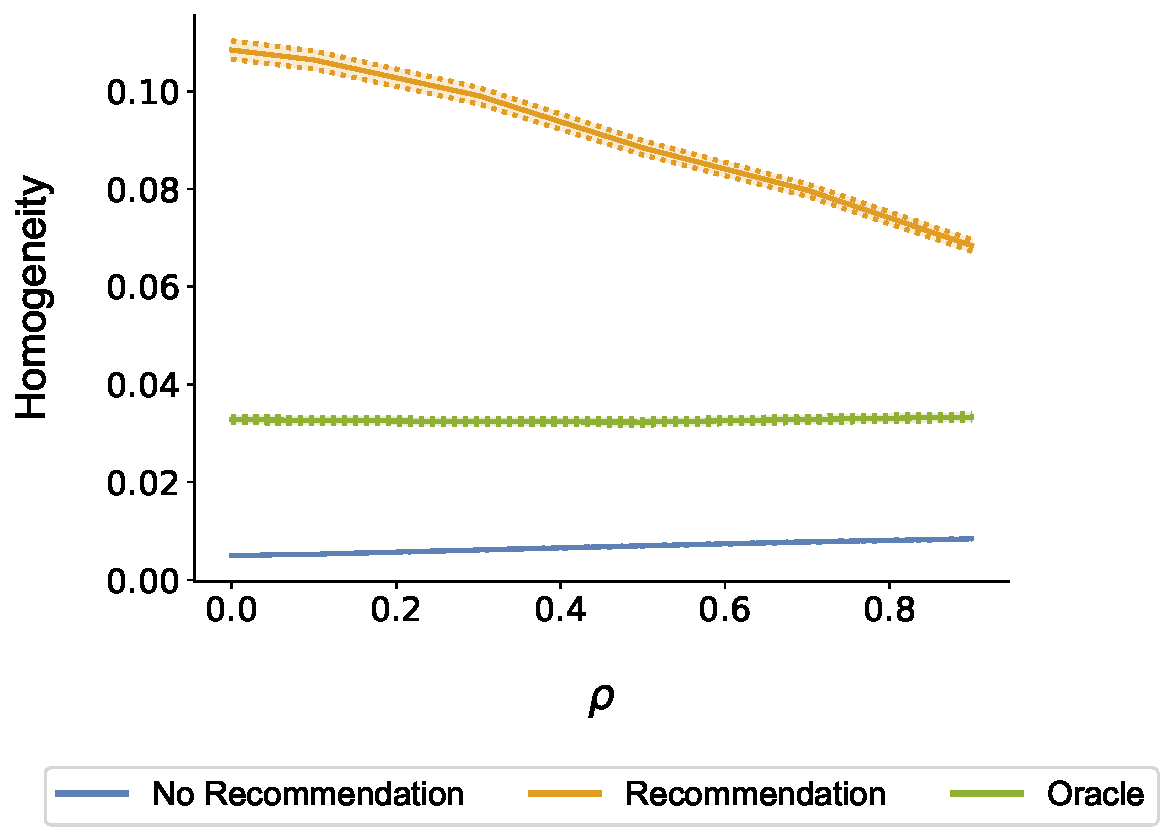
\includegraphics[width=.8\linewidth]{figures/rho_homogeneity_N_200_T_20}
\captionof{figure}{Correlation and Homogeneity}\label{fig:cor_homo}
\end{figure}

\section{Recommender System Evaluation}
In this section we discuss how the insights from our model of user decision-making can be used to inform the evaluation and design of recommender systems.
\par

The classic approach to recommender system evaluation is to predict user ratings for items and compare how accurate this prediction is to recorded ratings data, either explicitly given by users or inferred from behavioral data. Further, given this predicted rating, the recommender system should recommend to users the items with the highest predicted rating \cite{adomavicius2005toward}.
\par


There has been a recent movement away from such evaluation measures due to the observation that accurate recommendations are not necessarily useful recommendations \cite{mcnee2006being}. Our model illustrates why this could be the case. Consider the domain of movie recommendation and suppose a user has just watched the movie \textit{John Wick} and rated it highly. A recommender system attempting to predict user ratings may then predict that this user is very likely to enjoy the sequel, \textit{John Wick: Chapter Two}, as well. However, the user herself may also have made this inference since the two movies are very similar to each other and, after enjoying \textit{John Wick}, the user will update her beliefs about \textit{John Wick: Chapter Two}. Thus, if the recommender system recommends this movie to the user then this recommendation is not useful since the recommendation gives the user little information that they did not already know. The key insight is that the recommendation is not useful since \textit{it ignores the inference the user themselves made and their updated beliefs}. The user may watch \textit{John Wick: Chapter Two}, then, even without recommendation and the value of the recommendation was small.
\par

As a result, several alternative recommendation evaluation metrics, such as serendipity \cite{kotkov2016survey}, coverage \cite{ge2010beyond}, novelty \cite{vargas2011rank}, and many others have been proposed in order to develop recommender systems that produce recommendations that are more useful for users. We use our model to motivate an alternative recommendation evaluation metric that provides an alternative perspective on the serendipity metric proposed in the literature. Serendipitous recommendations are said to ``have the quality of being both unexpected and useful" \cite{maksai2015predicting} and we use this as a guide towards our definition.

Our approach to serendipity comes from the intuition that a recommendation is only useful insofar as it leads a user to take a better action than she would without recommendation. This approach stems from the idea that the value of recommendation is the marginal utility gain that a user receives from recommendation.\footnote{This notion is similar to the ``value of information" notion utilized in the literature in economics on the pricing of information goods \cite{bergemann2018design}.} This intuitively should come from providing information about products that, without additional information, users assign a low likelihood to being the best products currently available for them to consume and so would not consume them without these being recommended.
\par

This differs from other approaches in the literature since it depends on the beliefs of the users and what item the user would consume without recommendation. For instance, \cite{vargas2011rank, kaminskas2014measuring} propose unexpectedness metrics that look at the dissimilarity of the recommended items to what the recommender already knows the user likes either via a content-based approach or a collaborative-based approach. This depends only on the resulting item-set that the users get recommended and not necessarily user beliefs or the change in user action. \cite{adamopoulos2014unexpectedness} use an expected utility approach but use this to measure unexpectedness in terms of deviations from the ``expected consideration set" of a user and do not explicitly incorporate user beliefs.
\par

Our model allows us to give precise definitions for what it means for a recommendation to be \textit{unexpected} and \textit{useful}. Unexpected recommendations are given by recommended items that, given their beliefs, users have low expected utility from consuming, irregardless of what the true realized value is. Recall from Findings \ref{finding_local_consumption} and \ref{finding_diversity_welfare_corr} that, particularly if users are risk-averse, they will consume content in increasingly narrow portions of the product space and this may be detrimental to their realized welfare. As a result, identifying the portions of the product space where users may have significant uncertainty and utilizing recommendation to reduce this uncertainty can be welfare-enhancing for users. This is especially the case if this reduction of uncertainty leads users to explore under-explored portions of the product space where true realized utility is high, but expected utility, given beliefs, is low before recommendation.
\par

Useful recommendations are those that give users information that would change the item they consume relative to no recommendation and lead to an increase in expected utility given the updated beliefs when comparing the planned choice before and after the recommendation. In the previous example, recommending \textit{John Wick: Chapter Two} is not useful precisely because the expected utility before and after recommendation is the same since it does not change behavior. The most useful recommendations are those that (1) are informative given user beliefs and (2) induce users to consume unexpected goods.
\par

Operationalizing this approach requires the collection of data that is not traditionally collected for recommender systems. In particular, it becomes important to understand what choices users would make \textit{without recommendation} and to collect data on user beliefs, which can partially be inferred by observed choices. \cite{jiang2014choice, saavedra2016choice} argue that choice-based approaches alone can help in designing better RS, though they argue for these approaches because they do a better job at providing more accurate recommendations. Instead, we stress that choice-based approaches are useful not as recommendations but as a baseline for what recommendations would be useful.\footnote{Additionally, user beliefs and user choices contain information that may not have been observed by the recommender but is observed by the user. Ratings, reviews, friends, there are many sources of information affecting a person's beliefs and choices that are unobservable by recommender systems. Other consumption choices, e.g. movies seen in the cinema, change beliefs about for instance how good a director is, which affect beliefs about other movies and guide choices on a streaming platform that is unable to observe these data. However, this information can be inferred by the platform by collecting both beliefs and consumption choices.}
\par

Furthermore, our model shows the importance of understanding the underlying user preferences and the nature of the product space in the setting in which a recommender system is deployed since that will change the consumption patterns of users. For instance, understanding the degree of correlation of utilities and the level of risk-aversion become crucial in understanding how users will make consumption choices without recommendation and what kind of recommendation would be useful for users.
\par



\section{Conclusion}
We have studied a model of user decision-making in the context of markets where recommender systems are traditionally deployed in order to understand the consequences of recommender systems on consumption patterns of users. The key components of the model are that users make decisions under uncertainty and that consuming a good leads to informational spillovers about similar goods. We have shown that this alone can generate consumption behavior that is consistent with filter bubble effects that have traditionally been associated with personalized recommender systems. This effect is weakened once we allow for recommendation, but not as much as if users have full information. We have further explored the relationship between consumption diversity and user welfare and found that they are negatively correlated, implying that striving for consumption diversity is not necessarily welfare-improving for users. Finally, we have shown that recommendation can lead to increases in user homogenization both relative to no recommendation and full information since it concentrates users' consumption in portions of the product space with the highest utility according to the limits of what the recommender can predict about the utility of the good.
\par

We have used the insights from our model to guide the evaluation and design of recommender systems. The key insight is that a critical component of designing good recommendations is understanding what user behavior would be without recommendation and then understanding how recommendation would change their consumption. Operationalizing this requires collecting information on user beliefs about the goods in the product space, which is not data that is traditionally collected for the development of recommender systems.
\par

We leave for future work exploring to what extent user behavior changes if we drop the myopia assumption, so that users themselves are engaging in exploration. This likely interacts with recommendation in interesting ways as the recommendations may provide information that can complement or crowd-out user-led exploration. Our model also reveals a clear path-dependence in choice since consumption decisions today shape the information users have tomorrow about other products which affects their consumption choices tomorrow, etc. Even under the myopia assumption, understanding which recommendation system is optimal is an interesting and challenging problem.
\par

%We have argued that incorporating user choice under uncertainty should be a first-order component of RS design. By collecting appropriate data about user choices and user beliefs, RS can be built to better understand what choices users are likely to make and thus what information would be useful to give them as opposed to simply predicting what items a user will like. This approach can not only aid in designing more useful RS, but can also be utilized to better understand and prevent recently documented adverse effects of RS such as filter bubbles and homogenization.

%\newpage

%\subsection{User Homogenization}

%
%\begin{table}[bt]
%\centering
%\begin{tabular}{rlll}
%  \hline
%Rec Policy & Welfare & Diversity & Homogeneity \\ 
%  \hline
%No Rec & 0.42 $\pm$ 0.002 & 0.19 $\pm$ 0.0003 & 0.001 $\pm$ 0 \\ 
%Partial Rec & 1.25 $\pm$ 0.005 & 0.22 $\pm$ 0.0002 & 0.174 $\pm$ 0.004 \\ 
%Omniscient Rec & 2.24 $\pm$ 0.006 & 0.24 $\pm$ 0.0001 & 0.035 $\pm$ 0.002 \\ 
%   \hline
%\end{tabular}
%\caption{Mean Welfare, Diversity, and Homogeneity for $N = 1000, T = 25, I = 50, S = 50$. Reported intervals are 95\% confidence intervals.}
%\label{table:agg_results}
%\end{table}
%\begin{figure*}[!htbp]
%    \centering
%    \begin{minipage}[b]{0.5\textwidth}
%        \centering
%        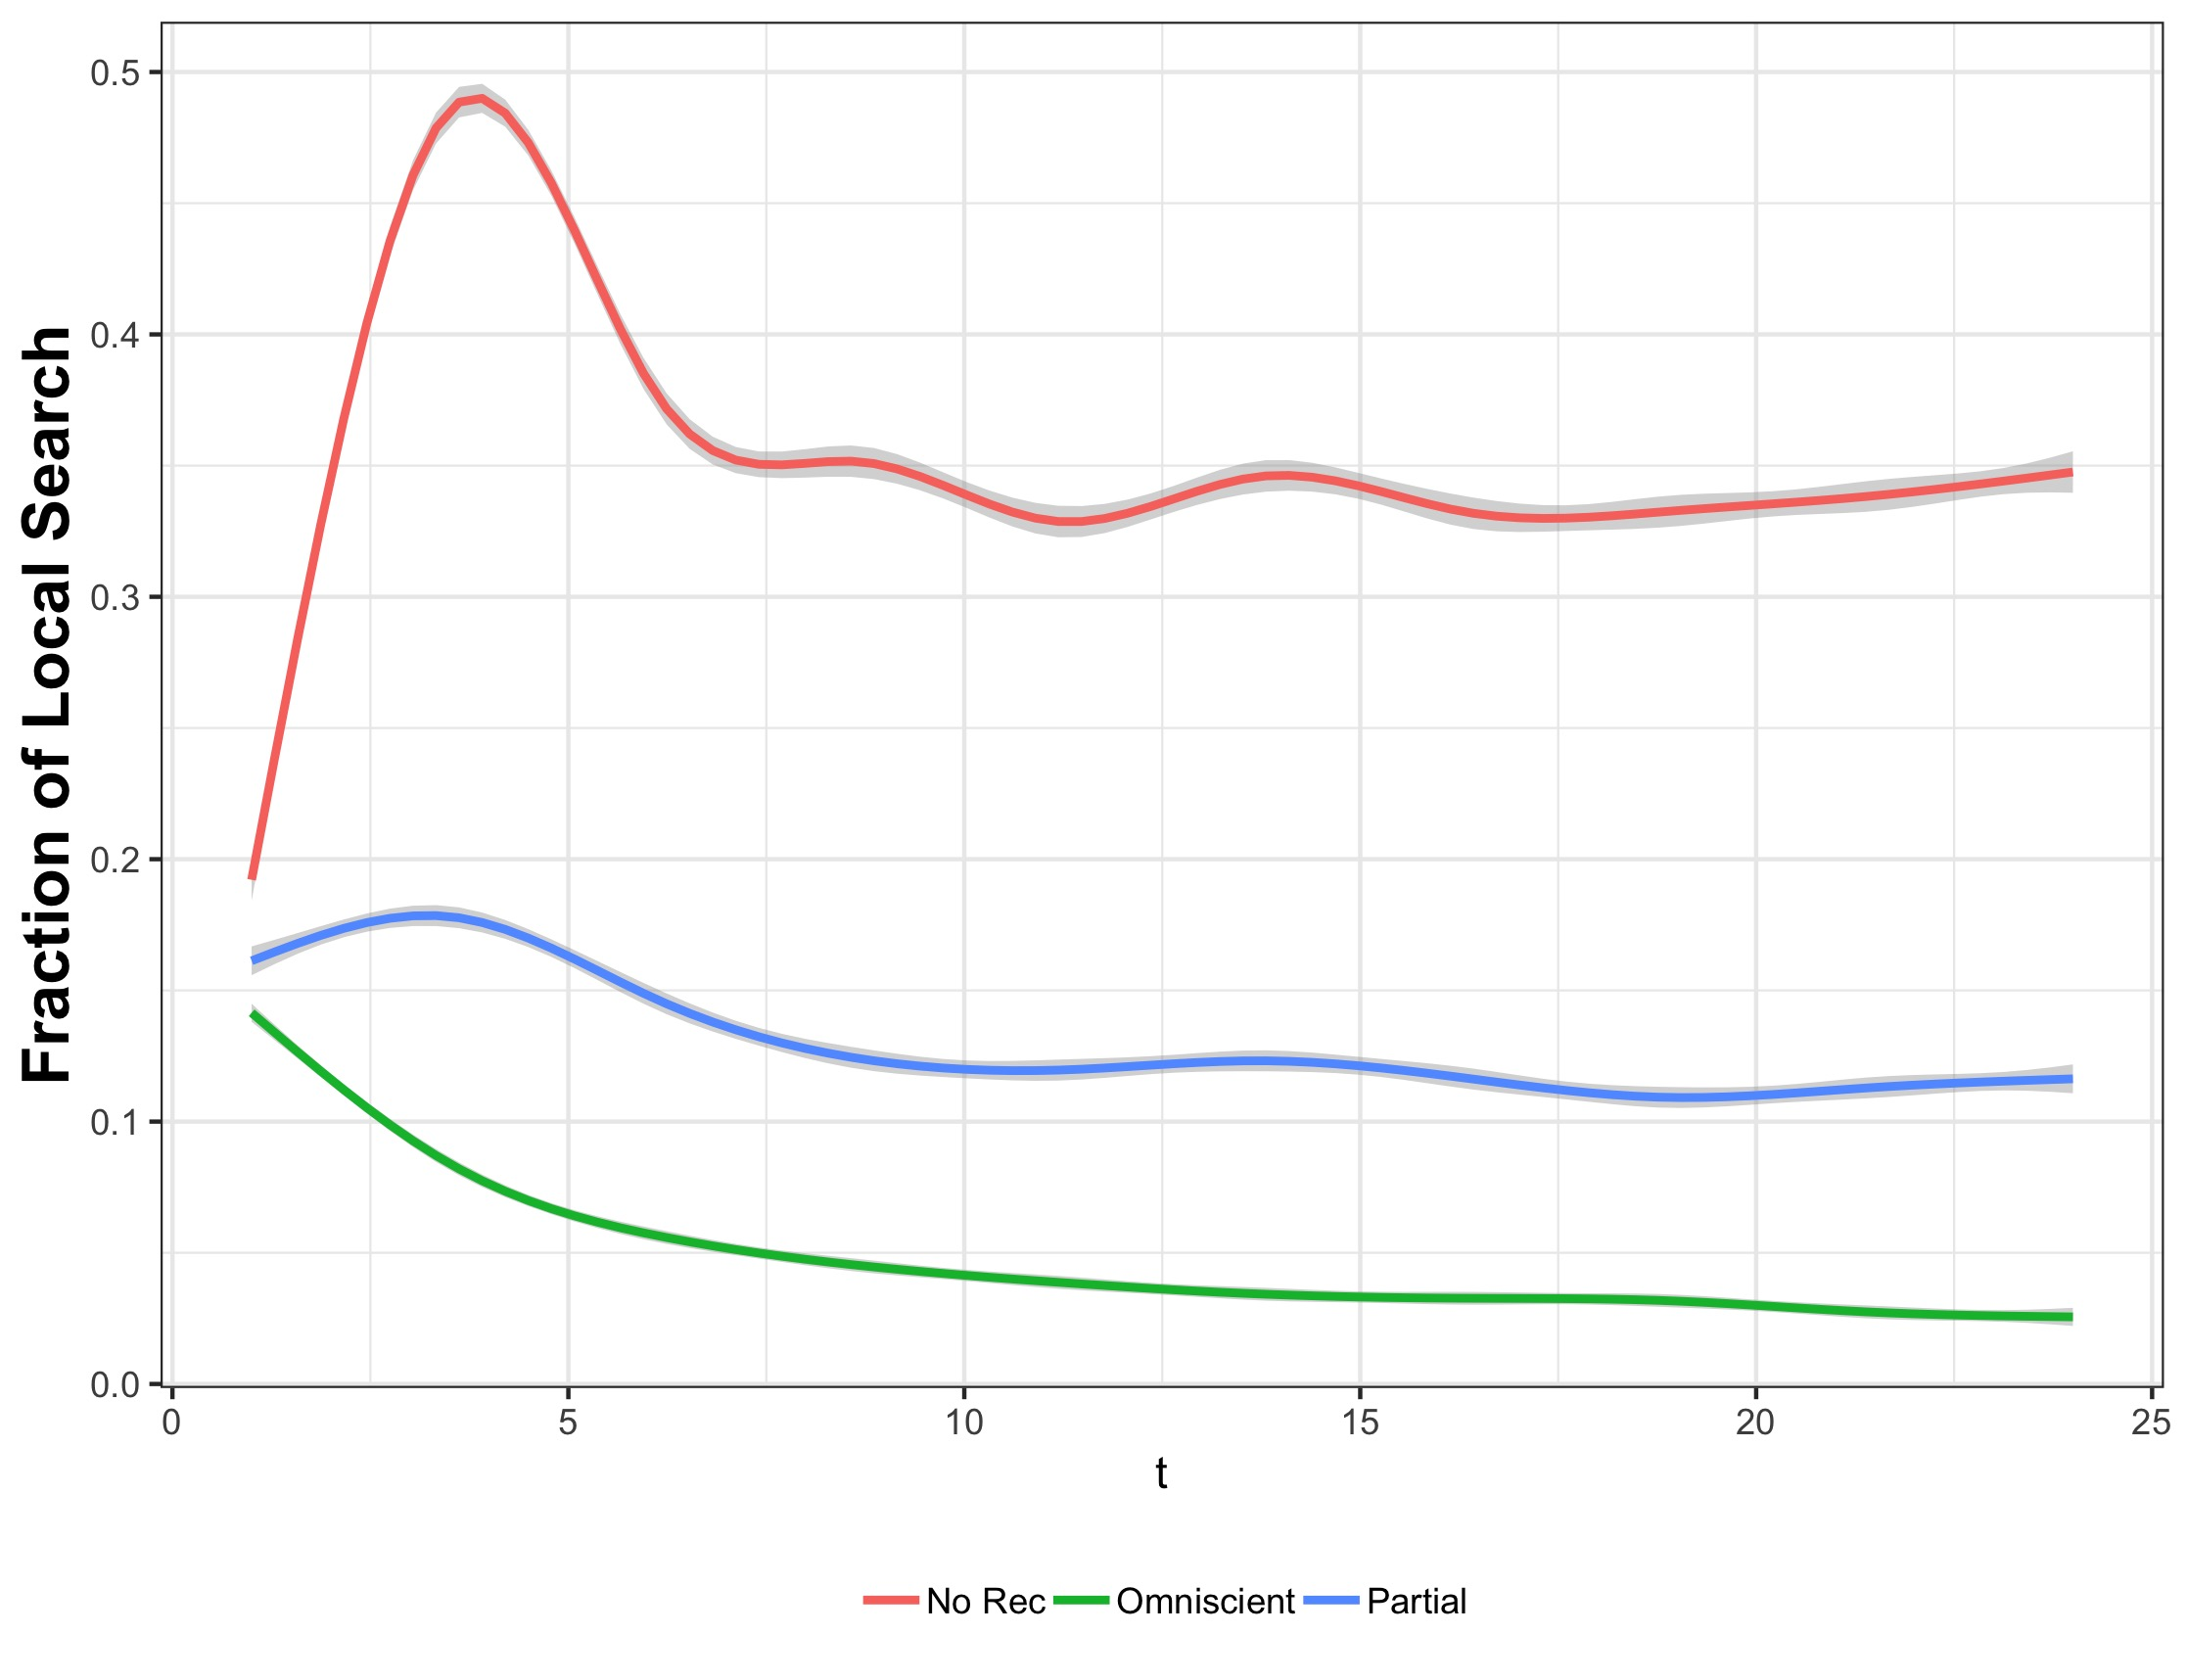
\includegraphics[width=0.9\linewidth, height=1.5in]{local_moves_25}
%        \caption{Extent of ``Local"  Consumption}
%        \label{fig:local_consumption}
%    \end{minipage}%
%    ~ 
%    \begin{minipage}[b]{0.5\textwidth}
%        \centering
%        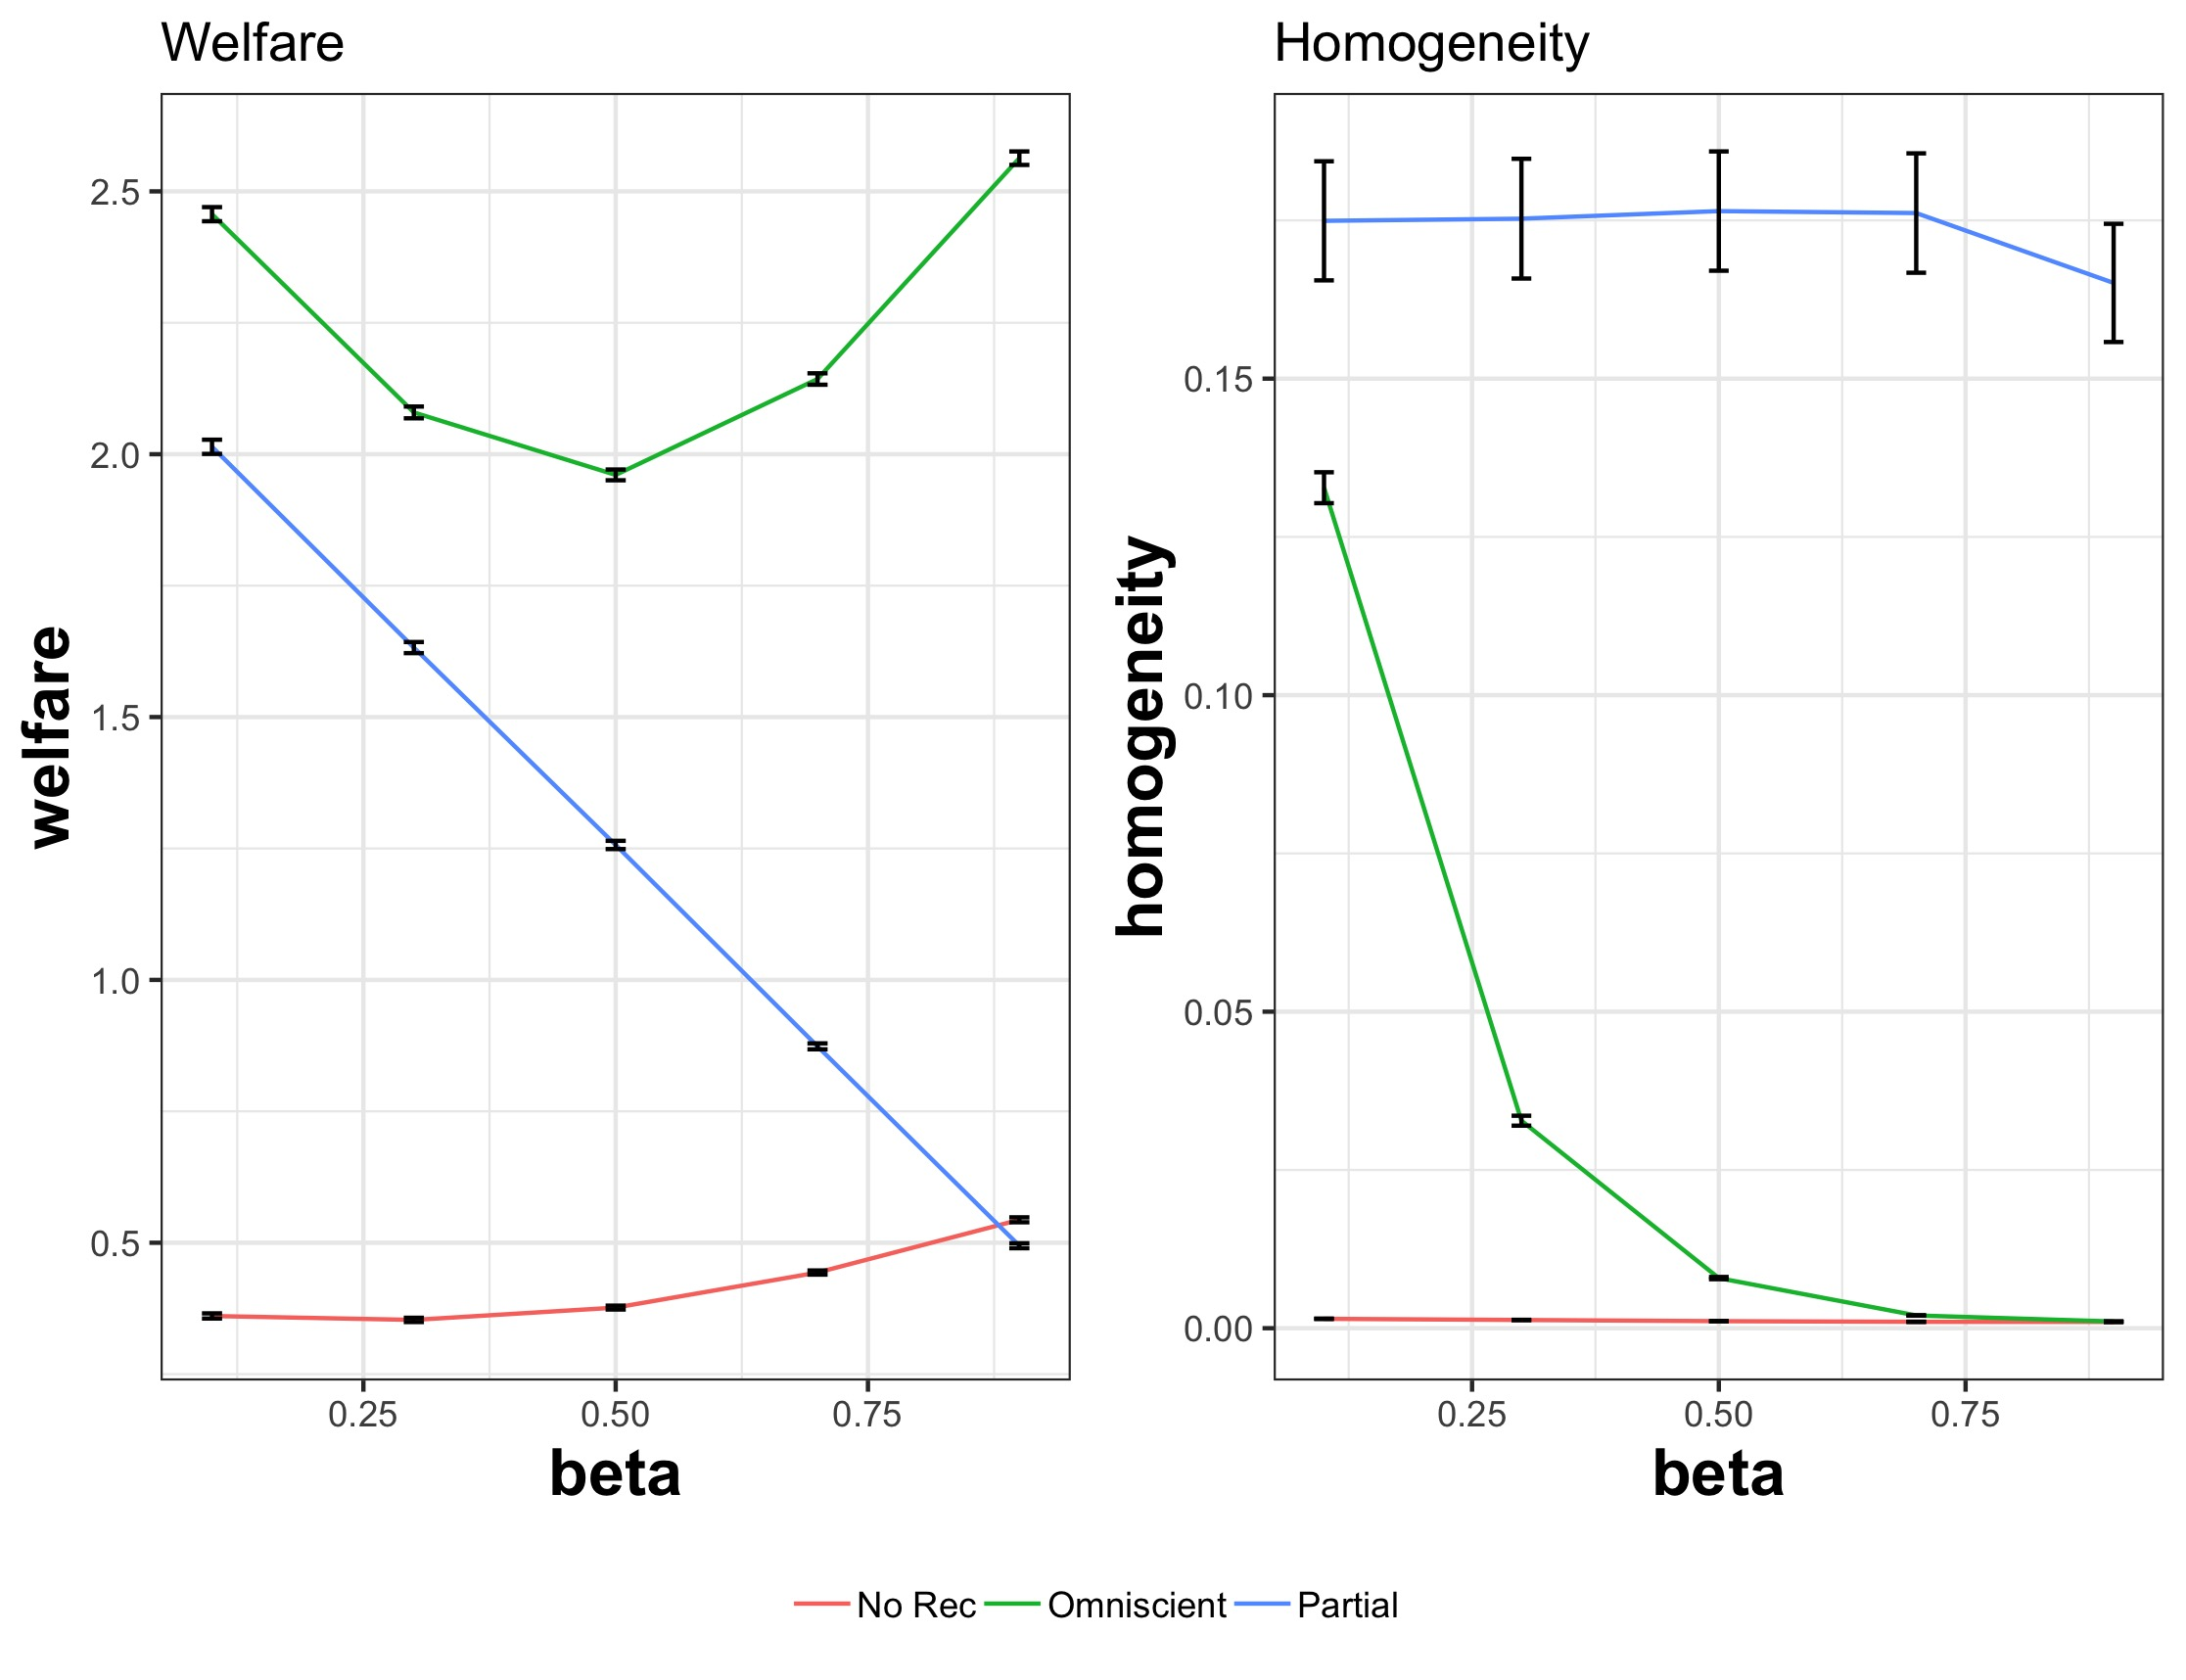
\includegraphics[width=0.9\linewidth, height=1.5in]{welfare_homo_combo}
%        \caption{Welfare and Homogeneity}
%        \label{fig:beta_vary}
%    \end{minipage}
%    ~ \\
%     \begin{minipage}{0.48\textwidth}
%     \centering
%     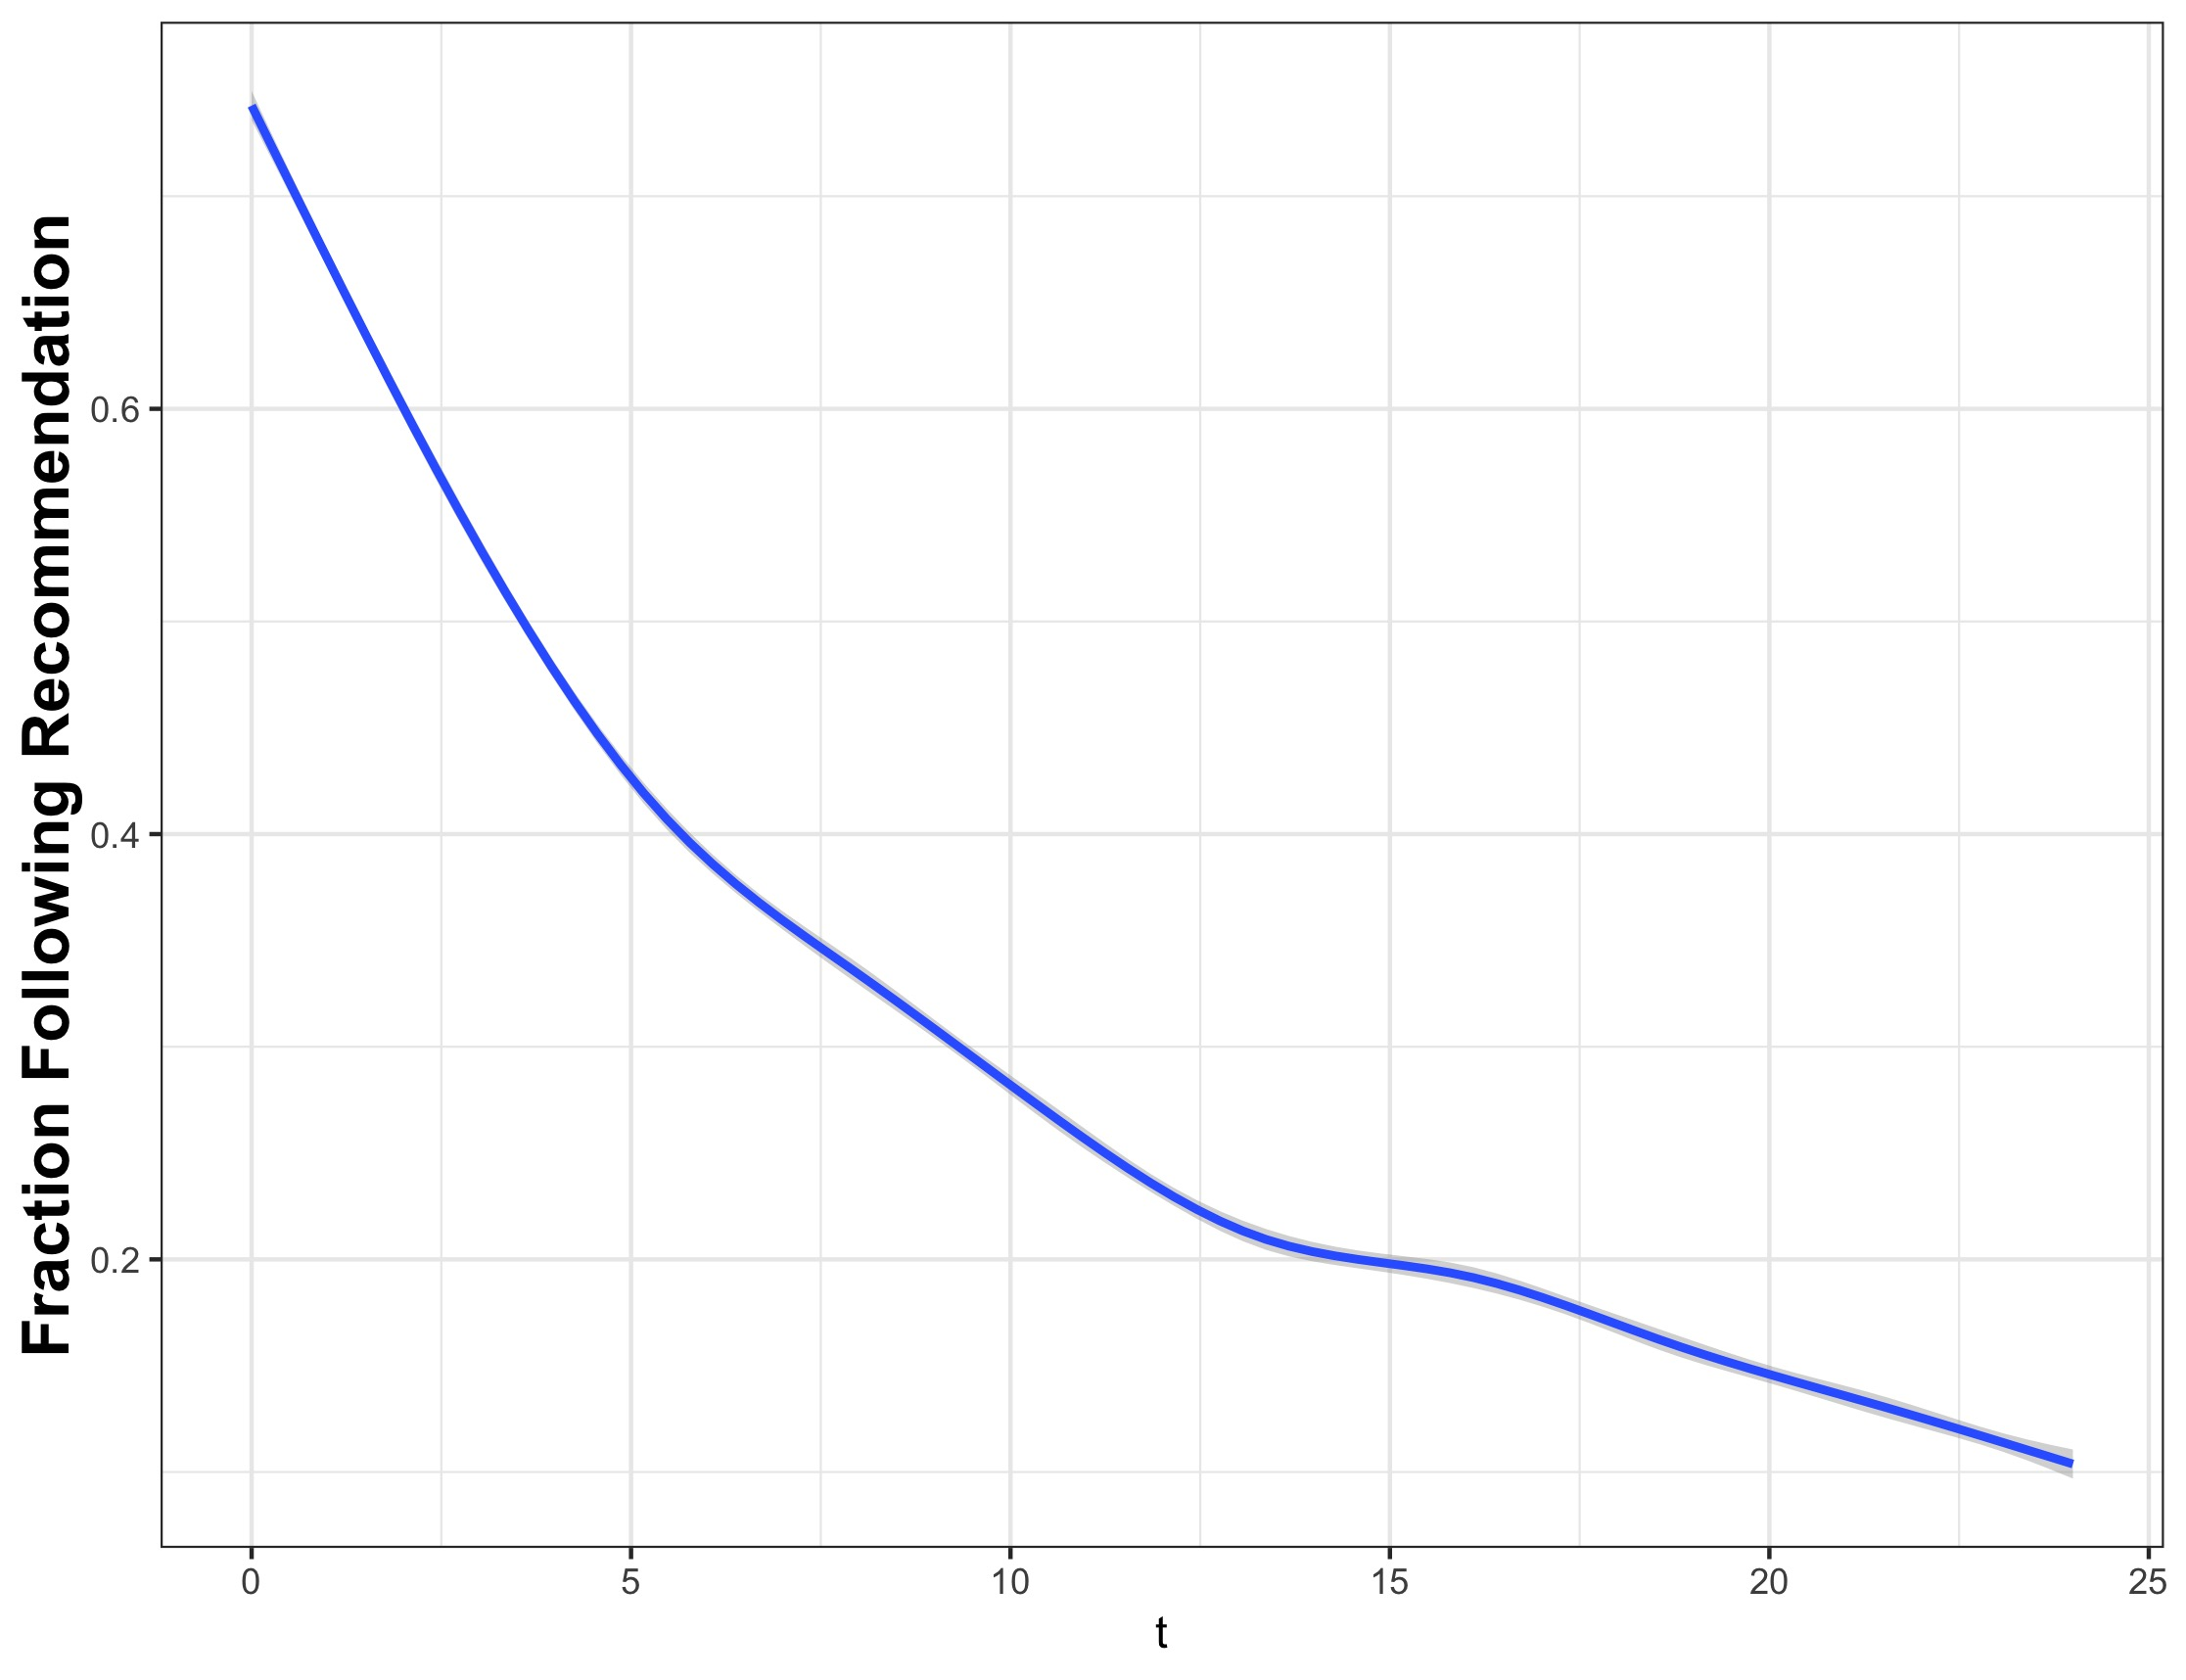
\includegraphics[width=0.9\linewidth, height=1.5in]{rec_obedience_25}
%     \caption{Recommendation Effectiveness}\label{fig:rec_obey}
%   \end{minipage}\hfill
%   ~
%   \begin{minipage}{0.48\textwidth}
%     \centering
%     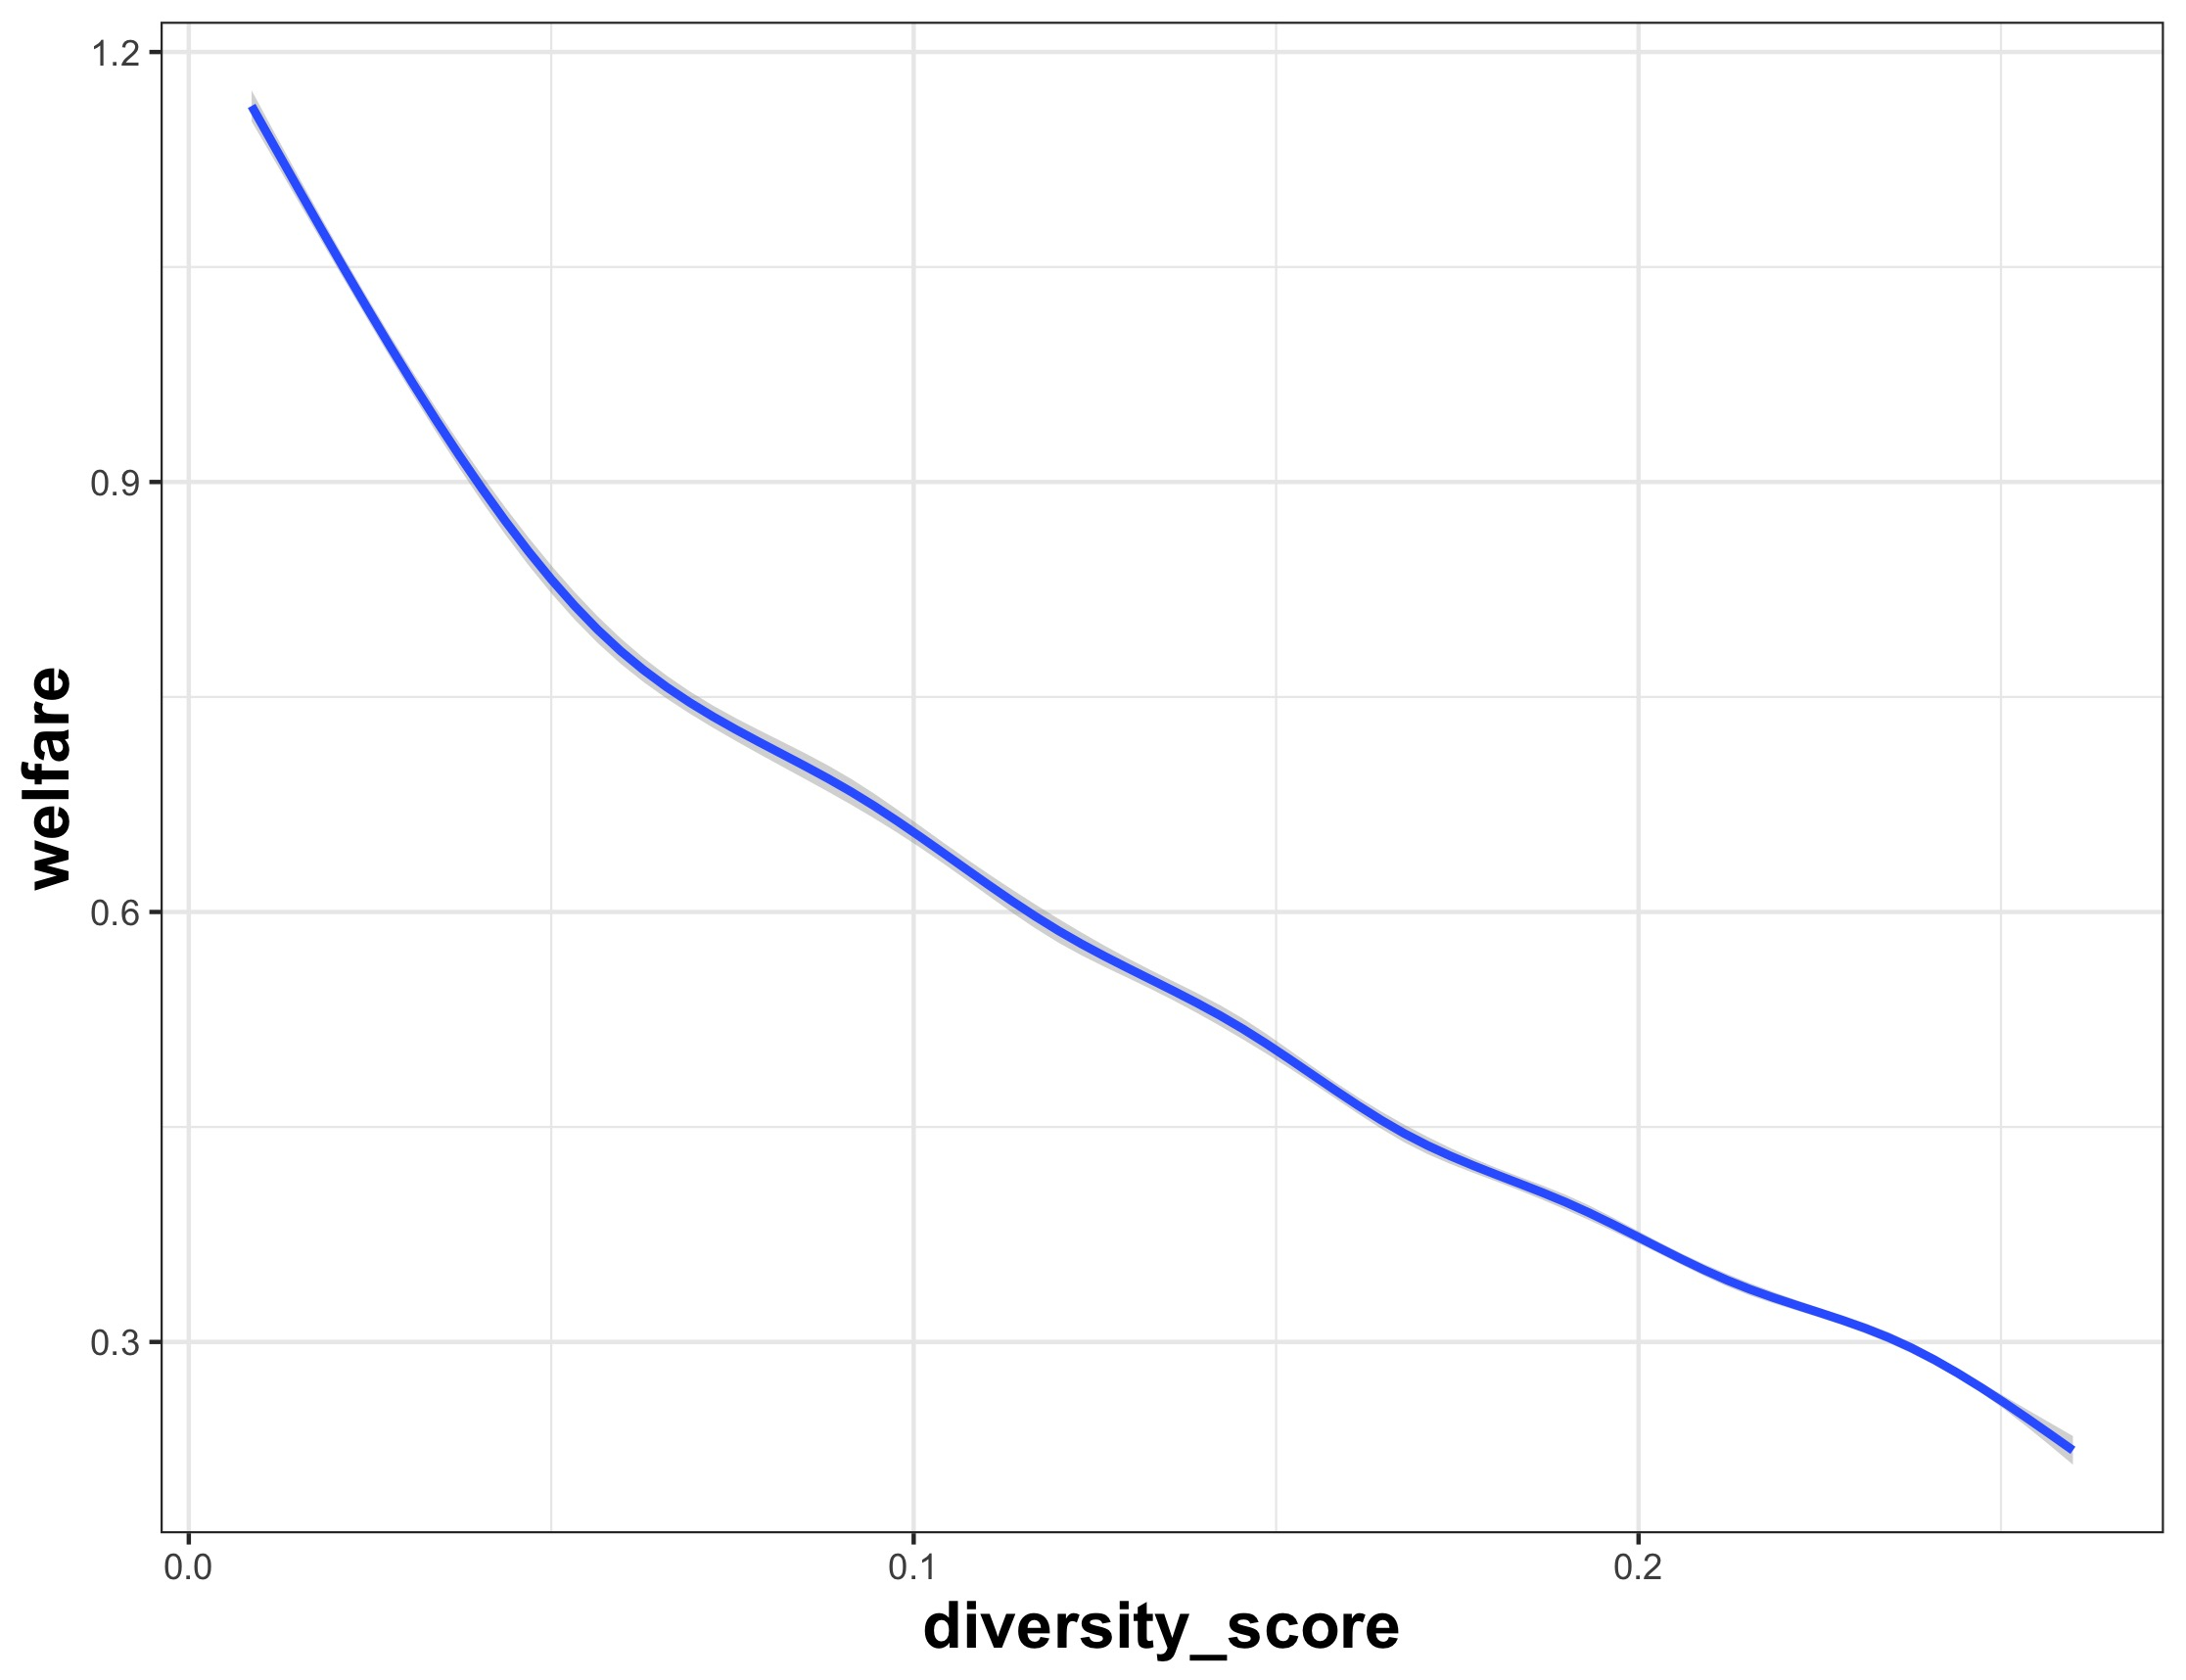
\includegraphics[width=0.9\linewidth, height=1.5in]{Diversity_vs_Welfare_No_Recommendation}
%     \caption{Diversity vs Welfare under No Recommendation}\label{fig:diversity_welfare_no_rec}
%   \end{minipage}
%\end{figure*}

%We are going to analyze three outcomes: how diverse consumer choices are, how similar are the choices that different individuals make and the resulting welfare. The first will be measured by $D_i =\frac{1}{N} \frac{1}{T (T-1)}\sum_{n,m \in C_i^T: n \ne m} d(n,m)$, the average normalized pairwise distance between the consumed products, a natural measure of diversity in this environment that is utilized in the literature \cite{ziegler2005improving}. The second will be measured by a consumer homogeneity index $H:=\frac{1}{|I|(|I|-1)}\sum_{i,j \in I: i \ne j}d_J(C_i^T,C_j^T) $, where $d_J$ denotes the Jaccard index and $H \in [0,1]$ which is similar to the approach to measuring homogeneity utilized in \cite{chaney2018algorithmic}. Note that a higher $H$ indicates more homogeneity. Consumer $i$'s welfare will just be the average of realized utilities, to control for the effect of $T$, $W_i=\frac{1}{T}\sum_{n \in C_i^T} u_{in}$.
%\par
%\par
%\noindent \textbf{Results}. Table \ref{table:agg_results} shows aggregate results for welfare, diversity, and homogeneity. The omniscient recommendation case leads to the optimal consumption path for a consumer since she consumes the $T$ items with the highest utility. Compared to this case, both partial recommendation and no recommendation not only lead to lower welfare but also have lower diversity. In fact, the no recommendation case leads to the lowest levels of consumption diversity since users do not explore the space of products sufficiently and do excessive amounts of local search as can be seen in Figure \ref{fig:local_consumption}. Figure \ref{fig:local_consumption} shows how ``local" consumption choices are by looking at what fraction of consecutive consumption choices are close to each other with the definition of close being less than distance of 10.  The partial recommendation case leads to higher consumption diversity and higher welfare, but also significantly higher homogeneity.
%
%In our model, filter bubble effects occur simply because of the correlation structure between the utility and beliefs of products. It highlights the fact that the correlation structure induces users to consume increasingly narrow content when they get no guidance from recommendation whereas the ``optimal" consumption path given by the omniscient policy does not exhibit this. The results of our model are consistent with the empirical results found in \cite{nguyen2014exploring} who show that filter bubble effects can arise even amongst users who do not utilize recommendations.
%\par
%Furthermore, \cite{nguyen2014exploring} also find that recommendation can lead to an increase in consumption diversity. As Table \ref{table:agg_results} shows, our model is consistent with this effect but it depends on the nature of recommendation. If recommendations only provides information on the common-value component (partially informed recommender) then welfare and consumption diversity increase when contrasted to the no recommendation case, but homogenization increases dramatically. Knowing the common-value component leads users to have more information on where to explore in the product space. However, the fact that this information is about the common-value component and the same across all individuals leads them to explore the same sections of the product space and leads to substantially higher homogeneity among users. If recommendation takes into account user beliefs on the idiosyncratic component of utility (omniscient recommender), then welfare and consumption diversity can further increase and homogeneity will decrease.
%\par
%Low consumption diversity is not necessarily bad by itself. Figure \ref{fig:diversity_welfare_no_rec} shows that, in the no recommendation case, welfare and consumption diversity are negatively correlated. This is primarily because content diversity in the no recommendation case can arise from the fact that the user consumes a bad product and is forced to jump around the product space looking for ``good" products. However, if a user finds a high utility product right away, then staying in this neighborhood may yield higher utility due to the correlation of utilities. The problem is that, even when the user finds a ``good" product, this may only be ``locally" good and the user will then excessively consume items around it due to having more information about these than more ``different'' ones, i.e. farther away.
%\par
%Finally, the value of recommendation in the partial recommendation case decreases over time as users learn more about the idiosyncratic component of their own preferences (i.e. as $t$ increases). Figure \ref{fig:rec_obey} shows that recommendation compliance decreases as $t$ increases. Additionally, Figure \ref{fig:beta_vary} shows how homogeneity and welfare change as $\beta$ increases. Most interestingly, when $\beta$ is high so that the common-value component is small, recommendation can be harmful to users. The information from recommendation still leads to large user homogeneity even though the optimum would be for there to be almost none and leads to lower welfare than under no recommendation.
%
%\section{The Value of the Ex-Ante View}
%
%In this section we illustrate the differences between the ex-post and ex-ante view and show how it is useful for thinking about the design of RS. Our first point is trivial to state - since users do not know the true consumption values of the items, without any further information they may make \textit{ex-post} sub-optimal consumption decisions, but \textit{ex-ante} optimal given the information available to them at the moment of choice. Consider the following stylized example. The choice set of the individual is $\Omega= \{x_1, x_2, x_3 \}$ and the ex-post utility values are given by
%$u(x_1) = 1$, $u(x_2) = 2$, $u(x_3) = 3$. 
%\par
%However, when users are making decisions they have unobservable \textit{beliefs} about the ex-post utility value of the items and make decisions given these beliefs. As users obtain more information, their beliefs converge to the ex-post utility values but, generally, users do not have enough information and so have beliefs over the space of possible ex-post utility values. In this example we suppose these beliefs are simple so that users view each good as simple lotteries: for $n=1,2,3$, $u(x_n) = n + \varepsilon_n$, $\varepsilon_1 \sim \mathcal J (2, 1)$, $\varepsilon_2 \sim \mathcal J (0, 1)$, $\varepsilon_3 \sim \mathcal J (-5, 2)$.
%\par
%After uncertainty is unresolved, the user would consume $x_3$, but an expected utility maximizing consumer (without further information) would choose $x_1$.\footnote{We ignore an important component of decision-making under uncertainty, risk attitudes, by focusing on risk-neutral consumers. A \textit{risk-averse} user may choose to consume a good with lower expected \textit{ex-post} payoff but lower ex-ante variance compared to another good. While risk-aversion is important for decision-making under uncertainty, especially in the context of RS, it is not our main focus here.}
%\par
%This observation, while seemingly trivial, has important implications. The fact that the user would choose $C$ over $A$ reveals that $C$ prefers $A$ given her current beliefs\footnote{This is a statement of \textit{revealed preference} which has been studied heavily in economic decision theory (see e.g. \cite[]{mas1995microeconomic}).} and allows the system designer to get some information about a user's beliefs. Why are user beliefs important objects for designers of RS to understand and utilize?
%\par
%Beliefs are useful for understanding how users interact and get value from RS. In particular, users use RS to get \textit{information} about the set of items and update their beliefs about the value of the items. For instance, in the example, a RS could recommend to a user $x_3$ over $x_2$ and $x_1$ and that user will use this to update her beliefs about $x_3$. It is an empirical question that we leave for future work precisely how and to what extent users update their beliefs from recommendation and what factors of RS deisgn influence this.\footnote{There has been some work in this direction in understanding when recommendations are persuasive \cite{cremonesi2012investigating, gretzel2006persuasion} as well as the effect of their delivery on effectiveness \cite{murphy2014recommendation}.}
%\par
%Better understanding user beliefs is important for improving the performance of RS that optimize for metrics that move away from accuracy such as serendipity \cite{kotkov2016survey}. Serendipity-based RS attempt to provide recommendations that ``have the quality of being both unexpected and useful" \cite{maksai2015predicting} but it is hard to know what items are both unexpected and useful \cite{kotkov2016survey}. Understanding \textit{why} a user has not consumed a good depends on the beliefs that the user has and this is important for designing serendipitious recommendations. For instance, in the example, the user does not consume $x_3$ because she expects the good to turn out worse than the other two. However, if given more information, she would prefer to consume it over $x_1$ and $x_2$. Moreover, when the user can use her known valuation of an item to make inferences on how good another item is, consumption is path-dependent, as beliefs guide consumption and consumption affects beliefs about other goods. For instance, learning the value of $x_1$ says something about how good $x_2$ is. %When considering risk-averse individuals, when the user has alternatives with a known value,The consumer may have also consumed Another reason why the user may not . The user may have an alternative with a known value -- say going for a walk around the neighborhood -- which she could always prefer to watching a given movie that has uncertain value but that the consumer thinks is always lower than the value of the walk.\footnote{An additional reason this could be useful is if one considers a risk-averse individual, then it may be that a user has not consumed an item because she has a high perceived variance for the item's quality.}
%As a result, understanding the beliefs of users helps us understand why users have not consumed certain items and, in particular, which items a user may find useful given more information about it. This poses an important problem: designing systems that elicit not only ex-post valuations but also ex-ante beliefs about valuations, as only by knowing these can RS be effective in steering users' choices. In particular, choice has to be perceived as guided by ex-ante utility, whereas ratings by the ex-post realized utility.
%\par
%Understanding the choices that individuals will make in addition to what they will end up liking are complementary problems but require different viewpoints. \cite{jiang2014choice, saavedra2016choice} argue that choice-based approaches alone can help in designing better RS, though they argue for these approaches because they do a better job at providing more accurate recommendations. We argue that the two problems should be considered separately -- though they may interact in interesting and useful ways.\footnote{In particular, some results in \cite{jiang2014choice, saavedra2016choice} may be driven by the fact that user choice embeds ratings information that may not have been observed by the recommender but is observed by the user. Ratings, reviews, friends, there are many sources of information affecting a person's beliefs and choices that are unobservable by RS. Other consumption choices, e.g. movies seen in the cinema, change beliefs about for instance how good a director is, which affect beliefs about other movies and guide choices on a streaming platform that is unable to observe these data.} 
%\par
%RS are designed to give users \textit{information} that is useful to help them make decisions. On the one hand, predicting a user's ex-post preferences is useful to know what items the user would like to consume. On the other hand, predicting what items a user will actually consume (without recommendation) can help reason about what information may actually be useful to give her. Furthermore, in designing RS to avoid filter bubble and homogenization effects, having accurate choice predictions allows mitigating such adverse effects to become a first-order component of design. In particular, by predicting both choice and ratings, RS can provide information to users that leads them to useful items but prevents them from falling into a filter bubble. 
%\par
%Solving this choice prediction problem requires data on the choices that individuals make and the sets that they choose them from in addition to the traditional ratings or behavioral data that is collected. In the example given previously the fact that the consumer chooses $x_1$ from the set $\{x_1, x_2, x_3 \}$ would be the data that is useful for the choice prediction problem, as would the consumer's ex-ante beliefs about her valuation of the goods.
%
%
%\section{Conclusion}
%
%We have argued that incorporating user choice under uncertainty should be a first-order component of RS design. By collecting appropriate data about user choices and user beliefs, RS can be built to better understand what choices users are likely to make and thus what information would be useful to give them as opposed to simply predicting what items a user will like. This approach can not only aid in designing more useful RS, but can also be utilized to better understand and prevent recently documented adverse effects of RS such as filter bubbles and homogenization.

\bibliographystyle{plain}
\bibliography{refs}
\end{document}
